\documentclass{article}
\usepackage{graphicx} % Required for inserting images
\usepackage{pgfplots}
\usepackage{tikz}
\usepackage{amsmath}
\usepackage{comment}
\usepackage{multicol}
\usepackage{float}
\usepackage{multicol}
\usepackage{hyperref}
\setlength{\columnsep}{0.75cm}
\RequirePackage[a4paper,margin=1.5cm]{geometry}

\hypersetup{
	colorlinks=true,
	linkcolor=violet,
}


\title{{\large Università degli Studi di Milano}\\{\large Corso di Laurea Triennale in Fisica}\\{\LARGE Esperienza di Millikan}\\{\normalsize Misura della carica dell'elettrone}}
\author{Carlo Moroni, Enco Musa, Matteo Pasolini\\{Turno: LU4}}
\date{October 14, 2024}

\begin{document}
	
\maketitle
\hrule
\begin{abstract}
	Abbiamo determinato la carica dell' elettrone misurando la velocità limite di goccioline di olio minerale cariche elettricamente, sia in assenza che in presenza di un campo elettrico.\\
	Il valore sperimentale ottenuto è $e=(1.64 \pm 0.03)\cdot10^{-19} C$, con una discrepanza di $1.09\sigma$ rispetto al valore universalmente accettato. 
\end{abstract}
\hrule

\section{Introduzione e modalità}

L'esperimento di Millikan si propone di misurare con precisione la carica elementare dell'elettrone, un parametro fondamentale per comprensione di numerosi fenomeni fisico-chimici. Questa esperienza ha inoltre fornito l'opportunità di osservare come le particelle cariche interagiscono con i campi elettrici.\\

Utilizzando un normale spruzzatore, sono state prodotte goccioline d'olio microscopiche, caricate elettricamente per strofinio, all'interno di una cameretta dotata di un condensatore. Attraverso un microscopio, dotato di reticolo, è stato possibile determinare la velocità di sedimentazione delle goccioline, misurando il loro tempo di volo e la distanza percorsa. Per ogni goccia, le misurazioni sono state effettuate inizialmente senza il campo elettrico, così da determinarne il raggio, e successivamente in presenza di campo elettrico, sia positivo che negativo, al fine di calcolare la carica elettrica depositata.

\section{Esposizione dei risultati}

Attraverso un'analisi preliminare dei dati, è possibile evidenziare alcuni aspetti significativi che hanno caratterizzato la misurazione della carica dell'elettrone.\\

In primo luogo, è importante sottolineare che le misurazioni sono risultate particolarmente complesse, principalmente causata dalla poca familiarità con lo strumento utilizzato. Inoltre, le difficoltà sono state aggravate dal comportamento imprevedibile delle gocce d'olio: in alcune occasioni, ne cadevano troppe simultaneamente, rendendo difficile la misurazione, mentre in altre, nessuna gocciolina era visibile, probabilmente a causa di un'ostruzione nella camera di Millikan. In altre situazioni, alcune goccioline non rispondevano al campo elettrico, sembrando quindi prive di carica, oppure risultavano troppo piccole e perciò soggette a moti irregolari e non rettilinei.\\

Le cariche misurate per le gocce numero 2 e numero 8, sia con campo positivo che negativo, non sono state incluse nel calcolo della carica dell'elettrone. Questo perché, analizzando i tempi di discesa e risalita registrati per entrambe le gocce, è emerso che tali valori risultavano incoerenti, essendo, spesso, inferiori a un secondo. Poiché il tempo di reazione umana è di circa 200 millisecondi e tendo conto anche del tempo necessario per comunicare l'avvio e l'arresto del cronometro, queste misurazioni non sono risultate affidabili.\\

Ulteriori cariche sono state escluse, in particolare quelle ottenute nelle prime misurazioni della goccia numero 5 (campo positivo), della goccia numero 7 (campo positivo) e della goccia numero 9 (campo positivo e negativo). Anche in questi casi, il primo tempo registrato è stato ritenuto inaffidabile poiché significativamente inferiore rispetto ai tempo misurati successivamente.\\

Infine, per quanto riguarda la goccia numero 3, non è stato possibile ottenere misurazioni con campo elettrico positivo, poiché la goccia stessa, dopo la misurazione in presenza di campo elettrico negativo, è scomparsa dal piano di osservazione, probabilmente interagendo con altre goccioline presenti.

\subsection{Goccia 1}
\begin{multicols}{2}
	
\begin{table}[H]
	\centering
	\begin{tabular}{| c | c |}
		\hline
		Resistenza [$M\Omega$] & $2.058$ \\
		\hline
		Temperatura [$^\circ C$] & $24$ \\
		\hline
		$\eta$ [$\frac{Ns}{m^2}$] & $1.843E-05$\\
		\hline
		$\eta_{eff}$ [$\frac{Ns}{m^2}$] & $1.473E-05$\\
		\hline
		$\Delta V$ [$V$] & $348$ \\
		\hline
		$E$ [$\frac N C$] & $46072$\\
		\hline
	\end{tabular}
	\caption{Tabella dei valori costanti all'interno della misurazione}
	\label{}
\end{table}

\columnbreak

\begin{table}[H]
	\centering
	\begin{tabular}{| c | c | c |}
		\hline
		$\Delta t$ [$s$] & $v$ [$\frac ms$] & $r$ [$m$] \\
		\hline
		$46.4$ & $1.078E-05$ & $2.878E-07$ \\
		$46.2$ & $1.083E-05$ & $2.886E-07$ \\
		$45.8$ & $1.092E-05$ & $2.900E-07$ \\
		$29.1$ & $1.720E-05$ & $3.731E-07$ \\
		$29.0$ & $1.725E-05$ & $3.738E-07$ \\
		\hline
	\end{tabular}
	\caption{Tabella dei tempi, velocità e raggi, misurati in assenza di campo elettrico}
	\label{}
\end{table}

\end{multicols}

\begin{multicols}{2}

\begin{table}[H]
	\centering
	\begin{tabular}{| c | c | c |}
		\hline
		$\Delta t$ [$s$] & $v$ [$\frac ms$] & $Q$ [$C$] \\
		\hline
		$2.0$ & $2.53E-04$ & $4.59E-19$ \\
		$1.5$ & $3.33E-04$ & $6.14E-19$ \\
		$1.8$ & $2.75E-04$ & $5.02E-19$ \\
		$1.7$ & $2.98E-04$ & $5.46E-19$ \\
		$2.1$ & $2.42E-04$ & $4.38E-19$ \\
		\hline
	\end{tabular}
	\caption{Tabella dei tempi, velocità e cariche, misurati in presenza di campo elettrico positivo}
	\label{}
\end{table}

\columnbreak

\begin{table}[H]
	\centering
	\begin{tabular}{| c | c | c |}
		\hline
		$\Delta t$ [$s$] & $v$ [$\frac ms$] & $Q$ [$C$] \\
		\hline
		$2.0$ & $2.50E-04$ & $5.06E-19$ \\
		$2.1$ & $2.40E-04$ & $4.87E-19$ \\
		$2.0$ & $2.46E-04$ & $4.99E-19$ \\
		$2.2$ & $2.29E-04$ & $4.66E-19$ \\
		$2.3$ & $2.22E-04$ & $4.52E-19$ \\
		\hline		
	\end{tabular}
	\caption{Tabella dei tempi, velocità e cariche, misurati in presenza di campo elettrico negativo}
	\label{}
\end{table}
	
\end{multicols}

\subsection{Goccia 2}

\begin{multicols}{2}

\begin{table}[H]
	\centering
	\begin{tabular}{| c | c |}
		\hline
		Resistenza [$M\Omega$] & $2.060$\\
		\hline
		Temperatura [$^\circ C$] & $24$\\
		\hline
		$\eta$ [$\frac{Ns}{m^2}$] & $1.843E-05$\\
		\hline
		$\eta_{eff}$ [$\frac{Ns}{m^2}$] & $1.494E-05$\\
		\hline
		$\Delta V$ [$V$] & $404$\\
		\hline
		$E$ [$\frac N C$] & $53486$\\
		\hline
	\end{tabular}
	\caption{Tabella dei valori costanti all'interno della misurazione}
	\label{}
\end{table}

\columnbreak

\begin{table}[H]
	\centering
	\begin{tabular}{| c | c | c |}
		\hline
		$\Delta t$ [$s$] & $v$ [$\frac ms$] & $r$ [$m$] \\
		\hline
		$35.0$ & $1.429E-05$ & $3.369E-07$ \\
		$36.4$ & $1.375E-05$ & $3.297E-07$ \\
		$29.5$ & $1.698E-05$ & $3.705E-07$ \\
		$32.3$ & $1.548E-05$ & $3.521E-07$ \\
		$33.6$ & $1.489E-05$ & $3.446E-07$ \\
		\hline
	\end{tabular}
	\caption{Tabella dei tempi, velocità e raggi, misurati in assenza di campo elettrico}
	\label{}
\end{table}
	
\end{multicols}

\begin{multicols}{2}

\begin{table}[H]
	\centering
	\begin{tabular}{| c | c | c |}
		\hline
		$\Delta t$ [$s$] & $v$ [$\frac ms$] & $Q$ [$C$] \\
		\hline
		$0.8$ & $6.17E-04$ & $1.10E-18$ \\
		$0.9$ & $5.81E-04$ & $1.03E-18$ \\
		$0.9$ & $5.88E-04$ & $1.05E-18$ \\
		$0.9$ & $5.56E-04$ & $9.86E-19$ \\
		$0.9$ & $5.81E-04$ & $1.03E-18$ \\
		\hline
	\end{tabular}
	\caption{Tabella dei tempi, velocità e cariche, misurati in presenza di campo elettrico positivo}
	\label{}
\end{table}

\columnbreak

\begin{table}[H]
	\centering
	\begin{tabular}{| c | c | c |}
		\hline
		$\Delta t$ [$s$] & $v$ [$\frac ms$] & $Q$ [$C$] \\
		\hline
		$1.0$ & $5.00E-04$ & $9.39E-19$ \\
		$1.0$ & $4.95E-04$ & $9.30E-19$ \\
		$0.9$ & $5.81E-04$ & $1.09E-18$ \\
		$0.9$ & $5.68E-04$ & $1.06E-18$ \\
		$0.9$ & $5.81E-04$ & $1.09E-18$ \\
		\hline		
	\end{tabular}
	\caption{Tabella dei tempi, velocità e cariche, misurati in presenza di campo elettrico negativo}
	\label{}
\end{table}
	
\end{multicols}

\subsection{Goccia 3}

\begin{multicols}{2}

\begin{table}[H]
	\centering
	\begin{tabular}{| c | c |}
		\hline
		Resistenza [$M\Omega$] & $2.058$\\
		\hline
		Temperatura [$^\circ C$] & $24$\\
		\hline
		$\eta$ [$\frac{Ns}{m^2}$] & $1.843E-05$\\
		\hline
		$\eta_{eff}$ [$\frac{Ns}{m^2}$] & $1.499E-05$\\
		\hline
		$\Delta V$ [$V$] & $306$\\
		\hline
		$E$ [$\frac N C$] & $40512$\\
		\hline
	\end{tabular}
	\caption{Tabella dei valori costanti all'interno della misurazione}
	\label{}
\end{table}

\columnbreak

\begin{table}[H]
	\centering
	\begin{tabular}{| c | c | c |}
		\hline
		$\Delta t$ [$s$] & $v$ [$\frac ms$] & $r$ [$m$] \\
		\hline
		$37.1$ & $1.348E-05$ & $3.262E-07$ \\
		$33.5$ & $1.493E-05$ & $3.451E-07$ \\
		$27.5$ & $1.817E-05$ & $3.845E-07$ \\
		$37.5$ & $1.334E-05$ & $3.243E-07$ \\
		$28.0$ & $1.789E-05$ & $3.812E-07$ \\
		\hline
	\end{tabular}
	\caption{Tabella dei tempi, velocità e raggi, misurati in assenza di campo elettrico}
	\label{}
\end{table}
	
\end{multicols}

\begin{multicols}{2}

Le misurazioni di questa goccia in presenza di campo elettrico positivo non è stato possibile prenderle in quanto la goccia stessa, dopo aver concluso la misurazione per il campo elettrico negativo, è scomparsa dal piano di osservazione, si suppone che abbia interagito con altre gocce presenti.

\columnbreak

\begin{table}[H]
	\centering
	\begin{tabular}{| c | c | c |}
		\hline
		$\Delta t$ [$s$] & $v$ [$\frac ms$] & $Q$ [$C$] \\
		\hline
		$5.1$ & $9.84E-05$ & $2.79E-19$ \\
		$4.6$ & $1.09E-04$ & $3.06E-19$ \\
		$4.6$ & $1.08E-04$ & $3.02E-19$ \\
		$4.5$ & $1.12E-04$ & $3.11E-19$ \\
		$3.6$ & $1.39E-04$ & $3.78E-19$ \\
		\hline		
	\end{tabular}
	\caption{Tabella dei tempi, velocità e cariche, misurati in presenza di campo elettrico negativo}
	\label{}
\end{table}
	
\end{multicols}

\subsection{Goccia 4}

\begin{multicols}{2}

\begin{table}[H]
	\centering
	\begin{tabular}{| c | c | c | c | c | c |}
		\hline
		Resistenza [$M\Omega$] & $2.023$\\
		\hline
		Temperatura [$^\circ C$]& $24$\\
		\hline
		$\eta$ [$\frac{Ns}{m^2}$] & $1.843E-05$\\
		\hline
		$\eta_{eff}$ [$\frac{Ns}{m^2}$] & $1.589E-05$\\
		\hline
		$\Delta V$ [$V$] & $340$\\
		\hline
		$E$ [$\frac N C$] & $45013$\\
		\hline
	\end{tabular}
	\caption{Tabella dei valori costanti all'interno della misurazione}
	\label{}
\end{table}

\columnbreak

\begin{table}[H]
	\centering
	\begin{tabular}{| c | c | c |}
		\hline
		$\Delta t$ [$s$] & $v$ [$\frac ms$] & $r$ [$m$] \\
		\hline
		$17.0$ & $2.948E-05$ & $4.999E-07$ \\
		$16.5$ & $3.023E-05$ & $5.067E-07$ \\
		$18.4$ & $2.720E-05$ & $4.787E-07$ \\
		$16.2$ & $3.092E-05$ & $5.129E-07$ \\
		$15.1$ & $3.311E-05$ & $5.321E-07$ \\
		\hline
	\end{tabular}
	\caption{Tabella dei tempi, velocità e raggi, misurati in assenza di campo elettrico}
	\label{}
\end{table}
	
\end{multicols}

\begin{multicols}{2}

\begin{table}[H]
	\centering
	\begin{tabular}{| c | c | c |}
		\hline
		$\Delta t$ [$s$] & $v$ [$\frac ms$] & $Q$ [$C$] \\
		\hline
		$3.7$ & $1.35E-04$ & $3.52E-19$ \\
		$4.0$ & $1.25E-04$ & $3.20E-19$ \\
		$3.9$ & $1.28E-04$ & $3.27E-19$ \\
		$3.6$ & $1.41E-04$ & $3.72E-19$ \\
		$4.1$ & $1.23E-04$ & $3.14E-19$ \\
		\hline
	\end{tabular}
	\caption{Tabella dei tempi, velocità e cariche, misurati in presenza di campo elettrico positivo}
	\label{}
\end{table}

\columnbreak

\begin{table}[H]
	\centering
	\begin{tabular}{| c | c | c |}
		\hline
		$\Delta t$ [$s$] & $v$ [$\frac ms$] & $Q$ [$C$] \\
		\hline
		$7.3$ & $6.84E-05$ & $3.32E-19$ \\
		$7.3$ & $6.89E-05$ & $3.33E-19$ \\
		$7.1$ & $7.06E-05$ & $3.39E-19$ \\
		$7.2$ & $6.96E-05$ & $3.36E-19$ \\
		$7.2$ & $6.98E-05$ & $3.36E-19$ \\
		\hline		
	\end{tabular}
	\caption{Tabella dei tempi, velocità e cariche, misurati in presenza di campo elettrico negativo}
	\label{}
\end{table}
	
\end{multicols}


\subsection{Goccia 5}

\begin{multicols}{2}

\begin{table}[H]
	\centering
	\begin{tabular}{| c | c | c | c | c | c |}
		\hline
		Resistenza [$M\Omega$] & $2.024$\\
		\hline
		Temperatura [$^\circ C$]& $24$\\
		\hline
		$\eta$ [$\frac{Ns}{m^2}$] & $1.843E-05$\\
		\hline
		$\eta_{eff}$ [$\frac{Ns}{m^2}$] & $1.624E-05$\\
		\hline
		$\Delta V$ [$V$] & $410$\\
		\hline
		$E$ [$\frac N C$] & $54281$\\
		\hline
	\end{tabular}
	\caption{Tabella dei valori costanti all'interno della misurazione}
	\label{}
\end{table}

\columnbreak

\begin{table}[H]
	\centering
	\begin{tabular}{| c | c | c |}
		\hline
		$\Delta t$ [$s$] & $v$ [$\frac ms$] & $r$ [$m$] \\
		\hline
		$12.6$ & $3.978E-05$ & $5.868E-07$ \\
		$11.9$ & $4.205E-05$ & $6.044E-07$ \\
		$12.2$ & $4.085E-05$ & $5.951E-07$ \\
		$11.9$ & $4.216E-05$ & $6.052E-07$ \\
		$11.4$ & $4.378E-05$ & $6.175E-07$ \\
		\hline
	\end{tabular}
	\caption{Tabella dei tempi, velocità e raggi, misurati in assenza di campo elettrico}
	\label{}
\end{table}
	
\end{multicols}

\begin{multicols}{2}

\begin{table}[H]
	\centering
	\begin{tabular}{| c | c | c |}
		\hline
		$\Delta t$ [$s$] & $v$ [$\frac ms$] & $Q$ [$C$] \\
		\hline
		$1.2$ & $4.17E-04$ & $1.27E-18$ \\
		$1.8$ & $2.86E-04$ & $8.28E-19$ \\
		$1.7$ & $2.91E-04$ & $8.45E-19$ \\
		$1.6$ & $3.13E-04$ & $9.19E-19$ \\
		$1.7$ & $3.03E-04$ & $8.87E-19$ \\
		\hline
	\end{tabular}
	\caption{Tabella dei tempi, velocità e cariche, misurati in presenza di campo elettrico positivo}
	\label{}
\end{table}

\columnbreak

\begin{table}[H]
	\centering
	\begin{tabular}{| c | c | c |}
		\hline
		$\Delta t$ [$s$] & $v$ [$\frac ms$] & $Q$ [$C$] \\
		\hline
		$2.1$ & $2.44E-04$ & $9.69E-19$ \\
		$2.4$ & $2.07E-04$ & $8.43E-19$ \\
		$2.1$ & $2.40E-04$ & $9.57E-19$ \\
		$2.7$ & $1.89E-04$ & $7.82E-19$ \\
		$2.4$ & $2.08E-04$ & $8.49E-19$ \\
		\hline		
	\end{tabular}
	\caption{Tabella dei tempi, velocità e cariche, misurati in presenza di campo elettrico negativo}
	\label{}
\end{table}
	
\end{multicols}

\subsection{Goccia 6}

\begin{multicols}{2}

\begin{table}[H]
	\centering
	\begin{tabular}{| c | c | c | c | c | c |}
		\hline
		Resistenza [$M\Omega$] & $2.028$\\
		\hline
		Temperatura [$^\circ C$]& $24$\\
		\hline
		$\eta$ [$\frac{Ns}{m^2}$] & $1.843E-05$\\
		\hline
		$\eta_{eff}$ [$\frac{Ns}{m^2}$] & $1.676E-05$\\
		\hline
		$\Delta V$ [$V$] & $380$\\
		\hline
		$E$ [$\frac N C$] & $50309$\\
		\hline
	\end{tabular}
	\caption{Tabella dei valori costanti all'interno della misurazione}
	\label{}
\end{table}

\columnbreak

\begin{table}[H]
	\centering
	\begin{tabular}{| c | c | c |}
		\hline
		$\Delta t$ [$s$] & $v$ [$\frac ms$] & $r$ [$m$] \\
		\hline
		$6.8$ & $7.386E-05$ & $8.134E-07$ \\
		$7.2$ & $6.983E-05$ & $7.899E-07$ \\
		$6.5$ & $7.692E-05$ & $8.309E-07$ \\
		$6.3$ & $7.937E-05$ & $8.446E-07$ \\
		$7.2$ & $6.983E-05$ & $7.899E-07$ \\
		\hline
	\end{tabular}
	\caption{Tabella dei tempi, velocità e raggi, misurati in assenza di campo elettrico}
	\label{}
\end{table}
	
\end{multicols}

\begin{multicols}{2}

\begin{table}[H]
	\centering
	\begin{tabular}{| c | c | c |}
		\hline
		$\Delta t$ [$s$] & $v$ [$\frac ms$] & $Q$ [$C$] \\
		\hline
		$1.4$ & $3.50E-04$ & $1.41E-18$ \\
		$1.5$ & $3.38E-04$ & $1.35E-18$ \\
		$1.7$ & $2.98E-04$ & $1.14E-18$ \\
		$1.7$ & $2.98E-04$ & $1.14E-18$ \\
		$1.5$ & $3.42E-04$ & $1.37E-18$ \\
		\hline
	\end{tabular}
	\caption{Tabella dei tempi, velocità e cariche, misurati in presenza di campo elettrico positivo}
	\label{}
\end{table}

\columnbreak

\begin{table}[H]
	\centering
	\begin{tabular}{| c | c | c |}
		\hline
		$\Delta t$ [$s$] & $v$ [$\frac ms$] & $Q$ [$C$] \\
		\hline
		$3.3$ & $1.50E-04$ & $1.14E-18$ \\
		$3.3$ & $1.53E-04$ & $1.16E-18$ \\
		$2.9$ & $1.74E-04$ & $1.27E-18$ \\
		$3.4$ & $1.49E-04$ & $1.14E-18$ \\
		$2.7$ & $1.87E-04$ & $1.33E-18$ \\
		\hline		
	\end{tabular}
	\caption{Tabella dei tempi, velocità e cariche, misurati in presenza di campo elettrico negativo}
	\label{}
\end{table}
	
\end{multicols}

\subsection{Goccia 7}

\begin{multicols}{2}

\begin{table}[H]
	\centering
	\begin{tabular}{| c | c | c | c | c | c |}
		\hline
		Resistenza [$M\Omega$] & $2.028$\\
		\hline
		Temperatura [$^\circ C$]& $24$\\
		\hline
		$\eta$ [$\frac{Ns}{m^2}$] & $1.843E-05$\\
		\hline
		$\eta_{eff}$ [$\frac{Ns}{m^2}$] & $1.672E-05$\\
		\hline
		$\Delta V$ [$V$] & $380$\\
		\hline
		$E$ [$\frac N C$] & $50309$\\
		\hline
	\end{tabular}
	\caption{Tabella dei valori costanti all'interno della misurazione}
	\label{}
\end{table}

\columnbreak

\begin{table}[H]
	\centering
	\begin{tabular}{| c | c | c |}
		\hline
		$\Delta t$ [$s$] & $v$ [$\frac ms$] & $r$ [$m$] \\
		\hline
		$7.6$ & $6.579E-05$ & $7.655E-07$ \\
		$7.2$ & $6.944E-05$ & $7.876E-07$ \\
		$7.2$ & $6.954E-05$ & $7.881E-07$ \\
		$6.6$ & $7.610E-05$ & $8.263E-07$ \\
		$7.0$ & $7.184E-05$ & $8.017E-07$ \\
		\hline
	\end{tabular}
	\caption{Tabella dei tempi, velocità e raggi, misurati in assenza di campo elettrico}
	\label{}
\end{table}
	
\end{multicols}

\begin{multicols}{2}

\begin{table}[H]
	\centering
	\begin{tabular}{| c | c | c |}
		\hline
		$\Delta t$ [$s$] & $v$ [$\frac ms$] & $Q$ [$C$] \\
		\hline
		$1.3$ & $3.85E-04$ & $1.56E-18$ \\
		$1.6$ & $3.07E-04$ & $1.17E-18$ \\
		$1.6$ & $3.23E-04$ & $1.25E-18$ \\
		$1.6$ & $3.13E-04$ & $1.20E-18$ \\
		$1.5$ & $3.38E-04$ & $1.33E-18$ \\
		\hline
	\end{tabular}
	\caption{Tabella dei tempi, velocità e cariche, misurati in presenza di campo elettrico positivo}
	\label{}
\end{table}

\columnbreak

\begin{table}[H]
	\centering
	\begin{tabular}{| c | c | c |}
		\hline
		$\Delta t$ [$s$] & $v$ [$\frac ms$] & $Q$ [$C$] \\
		\hline
		$2.7$ & $1.87E-04$ & $1.28E-18$ \\
		$2.9$ & $1.74E-04$ & $1.22E-18$ \\
		$2.5$ & $2.02E-04$ & $1.35E-18$ \\
		$2.8$ & $1.79E-04$ & $1.24E-18$ \\
		$2.5$ & $2.04E-04$ & $1.37E-18$ \\
		\hline		
	\end{tabular}
	\caption{Tabella dei tempi, velocità e cariche, misurati in presenza di campo elettrico negativo}
	\label{}
\end{table}
	
\end{multicols}


\subsection{Goccia 8}

\begin{multicols}{2}

\begin{table}[H]
	\centering
	\begin{tabular}{| c | c | c | c | c | c |}
		\hline
		Resistenza [$M\Omega$] & $2.029$\\
		\hline
		Temperatura [$^\circ C$]& $24$\\
		\hline
		$\eta$ [$\frac{Ns}{m^2}$] & $1.843E-05$\\
		\hline
		$\eta_{eff}$ [$\frac{Ns}{m^2}$] & $1.633E-05$\\
		\hline
		$\Delta V$ [$V$] & $410$\\
		\hline
		$E$ [$\frac N C$] & $54281$\\
		\hline
	\end{tabular}
	\caption{Tabella dei valori costanti all'interno della misurazione}
	\label{}
\end{table}

\columnbreak

\begin{table}[H]
	\centering
	\begin{tabular}{| c | c | c |}
		\hline
		$\Delta t$ [$s$] & $v$ [$\frac ms$] & $r$ [$m$] \\
		\hline
		$11.4$ & $4.390E-05$ & $6.183E-07$ \\
		$11.7$ & $4.292E-05$ & $6.110E-07$ \\
		$10.7$ & $4.686E-05$ & $6.401E-07$ \\
		$9.5$ & $5.258E-05$ & $6.803E-07$ \\
		$12.0$ & $4.156E-05$ & $6.006E-07$ \\
		\hline
	\end{tabular}
	\caption{Tabella dei tempi, velocità e raggi, misurati in assenza di campo elettrico}
	\label{}
\end{table}
	
\end{multicols}

\begin{multicols}{2}

\begin{table}[H]
	\centering
	\begin{tabular}{| c | c | c |}
		\hline
		$\Delta t$ [$s$] & $v$ [$\frac ms$] & $Q$ [$C$] \\
		\hline
		$0.9$ & $4.95E-04$ & $1.60E-18$ \\
		$0.8$ & $4.95E-04$ & $1.60E-18$ \\
		$0.8$ & $4.95E-04$ & $1.60E-18$ \\
		$0.9$ & $4.95E-04$ & $1.60E-18$ \\
		$0.8$ & $4.95E-04$ & $1.60E-18$ \\
		\hline
	\end{tabular}
	\caption{Tabella dei tempi, velocità e cariche, misurati in presenza di campo elettrico positivo}
	\label{}
\end{table}

\columnbreak

\begin{table}[H]
	\centering
	\begin{tabular}{| c | c | c |}
		\hline
		$\Delta t$ [$s$] & $v$ [$\frac ms$] & $Q$ [$C$] \\
		\hline
		$1.0$ & $4.95E-04$ & $1.93E-18$ \\
		$1.0$ & $4.95E-04$ & $1.93E-18$ \\
		$1.0$ & $4.95E-04$ & $1.93E-18$ \\
		$1.0$ & $4.95E-04$ & $1.93E-18$ \\
		$1.0$ & $4.95E-04$ & $1.93E-18$ \\
		\hline		
	\end{tabular}
	\caption{Tabella dei tempi, velocità e cariche, misurati in presenza di campo elettrico negativo}
	\label{}
\end{table}
	
\end{multicols}

\subsection{Goccia 9}

\begin{multicols}{2}

\begin{table}[H]
	\centering
	\begin{tabular}{| c | c | c | c | c | c |}
		\hline
		Resistenza [$M\Omega$] & $2.025$\\
		\hline
		Temperatura [$^\circ C$]& $24$\\
		\hline
		$\eta$ [$\frac{Ns}{m^2}$] & $1.843E-05$\\
		\hline
		$\eta_{eff}$ [$\frac{Ns}{m^2}$] & $1.609E-05$\\
		\hline
		$\Delta V$ [$V$] & $306$\\
		\hline
		$E$ [$\frac N C$] & $40512$\\
		\hline
	\end{tabular}
	\caption{Tabella dei valori costanti all'interno della misurazione}
	\label{}
\end{table}

\columnbreak

\begin{table}[H]
	\centering
	\begin{tabular}{| c | c | c |}
		\hline
		$\Delta t$ [$s$] & $v$ [$\frac ms$] & $r$ [$m$] \\
		\hline
		$16.8$ & $2.971E-05$ & $5.020E-07$ \\
		$12.9$ & $3.891E-05$ & $5.799E-07$ \\
		$13.9$ & $3.597E-05$ & $5.561E-07$ \\
		$13.0$ & $3.849E-05$ & $5.766E-07$ \\
		$13.3$ & $3.754E-05$ & $5.689E-07$ \\
		\hline
	\end{tabular}
	\caption{Tabella dei tempi, velocità e raggi, misurati in assenza di campo elettrico}
	\label{}
\end{table}
	
\end{multicols}

\begin{multicols}{2}

\begin{table}[H]
	\centering
	\begin{tabular}{| c | c | c |}
		\hline
		$\Delta t$ [$s$] & $v$ [$\frac ms$] & $Q$ [$C$] \\
		\hline
		$4.0$ & $1.24E-04$ & $3.64E-19$ \\
		$2.5$ & $2.04E-04$ & $6.98E-19$ \\
		$3.0$ & $1.67E-04$ & $5.43E-19$ \\
		$3.3$ & $1.52E-04$ & $4.80E-19$ \\
		$2.6$ & $1.90E-04$ & $6.40E-19$ \\
		\hline
	\end{tabular}
	\caption{Tabella dei tempi, velocità e cariche, misurati in presenza di campo elettrico positivo}
	\label{}
\end{table}

\columnbreak

\begin{table}[H]
	\centering
	\begin{tabular}{| c | c | c |}
		\hline
		$\Delta t$ [$s$] & $v$ [$\frac ms$] & $Q$ [$C$] \\
		\hline
		$8.8$ & $5.66E-05$ & $3.85E-19$ \\
		$3.8$ & $1.31E-04$ & $6.96E-19$ \\
		$5.8$ & $8.64E-05$ & $5.09E-19$ \\
		$5.3$ & $9.38E-05$ & $5.40E-19$ \\
		$3.9$ & $1.28E-04$ & $6.83E-19$ \\
		\hline		
	\end{tabular}
	\caption{Tabella dei tempi, velocità e cariche, misurati in presenza di campo elettrico negativo}
	\label{}
\end{table}
	
\end{multicols}

\subsection{Goccia 10}
\begin{multicols}{2}

\begin{table}[H]
	\centering
	\begin{tabular}{| c | c | c | c | c | c |}
		\hline
		Resistenza [$M\Omega$] & $2.028$\\
		\hline
		Temperatura [$^\circ C$]& $24$\\
		\hline
		$\eta$ [$\frac{Ns}{m^2}$] & $1.843E-05$\\
		\hline
		$\eta_{eff}$ [$\frac{Ns}{m^2}$] & $1.661E-05$\\
		\hline
		$\Delta V$ [$V$] & $410$\\
		\hline
		$E$ [$\frac N C$] & $54281$\\
		\hline
	\end{tabular}
	\caption{Tabella dei valori costanti all'interno della misurazione}
	\label{}
\end{table}

\columnbreak

\begin{table}[H]
	\centering
	\begin{tabular}{| c | c | c |}
		\hline
		$\Delta t$ [$s$] & $v$ [$\frac ms$] & $r$ [$m$] \\
		\hline
		$8.7$ & $5.760E-05$ & $7.139E-07$ \\
		$8.5$ & $5.896E-05$ & $7.227E-07$ \\
		$7.7$ & $6.468E-05$ & $7.587E-07$ \\
		$7.5$ & $6.693E-05$ & $7.725E-07$ \\
		$8.5$ & $5.910E-05$ & $7.236E-07$ \\
		\hline
	\end{tabular}
	\caption{Tabella dei tempi, velocità e raggi, misurati in assenza di campo elettrico}
	\label{}
\end{table}ur account safe and
	
\end{multicols}

\begin{multicols}{2}

\begin{table}[H]
	\centering
	\begin{tabular}{| c | c | c |}
		\hline
		$\Delta t$ [$s$] & $v$ [$\frac ms$] & $Q$ [$C$] \\
		\hline
		$2.1$ & $2.36E-04$ & $7.42E-19$ \\
		$1.9$ & $2.70E-04$ & $8.88E-19$ \\
		$2.1$ & $2.42E-04$ & $7.66E-19$ \\
		$1.7$ & $2.92E-04$ & $9.82E-19$ \\
		$2.1$ & $2.40E-04$ & $7.61E-19$ \\
		\hline
	\end{tabular}
	\caption{Tabella dei tempi, velocità e cariche, misurati in presenza di campo elettrico positivo}
	\label{}
\end{table}

\columnbreak

\begin{table}[H]
	\centering
	\begin{tabular}{| c | c | c |}
		\hline
		$\Delta t$ [$s$] & $v$ [$\frac ms$] & $Q$ [$C$] \\
		\hline
		$4.1$ & $1.23E-04$ & $7.84E-19$ \\
		$3.9$ & $1.29E-04$ & $8.11E-19$ \\
		$3.9$ & $1.27E-04$ & $8.03E-19$ \\
		$3.8$ & $1.32E-04$ & $8.21E-19$ \\
		$3.9$ & $1.28E-04$ & $8.07E-19$ \\
		\hline		
	\end{tabular}
	\caption{Tabella dei tempi, velocità e cariche, misurati in presenza di campo elettrico negativo}
	\label{}
\end{table}
	
\end{multicols}

\section{Analisi dei dati}
Attraverso un'analisi preliminare dei dati, è possibile evidenziare alcuni aspetti significativi che hanno caratterizzato la misurazione della carica dell'elettrone.\\

In primo luogo, è importante sottolineare che le misurazioni sono risultate particolarmente complesse, principalmente causata dalla poca familiarità con lo strumento utilizzato. Inoltre, le difficoltà sono state aggravate dal comportamento imprevedibile delle gocce d'olio: in alcune occasioni, ne cadevano troppe simultaneamente, rendendo difficile la misurazione, mentre in altre, nessuna gocciolina era visibile, probabilemente a causa di un'ostruzione nella camera di Millikan. In altre situazioni, alcune goccioline non rispondevano al campo elettrico, sembrando quindi prive di carica, oppure risultavano troppo piccole e perciò soggette a moti irregolari e non rettilinei.\\

Le cariche misurate per le gocce numero 2 e numero 8, sia con campo positivo che negativo, non sono state incluse nel calcolo della carica dell'elettrone. Questo perché, analizzando i tempi di discesa e risalita registrati per entrambe le gocce, è emerso che tali valori risultavano incoerenti, essendo, spesso, inferiori a un secondo. Poichè il tempo di reazione umana è di circa 200 milli secondi e tendo conto anche del tempo necessario per comunicare l'avvio e l'arresto del cronometro, queste misurazioni non sono risultate affidabili.\\

Ulteriori cariche sono state escluse, in particolare quelle ottenute nelle prime misurazioni della goccia numero 5 (campo positivo), della goccia numero 7 (campo positivo) e della goccia numero 9 (campo positivo e negativo). Anche in questi casi, il primo tempo registrato è stato ritenuto inaffidabile poichè significativamente inferiore rispetto ai tempo misurati successivamente.\\

Infine, per quanto riguarda la goccia numero 3, non è stato possibile ottenere misurazioni con campo elettrico positivo, poichè la goccia stessa, dopo la misurazione in presenza di campo elettrico negativo, è scomparssa dal piano di osservazione, probabilmente interagendo con altre goccioline presenti.

\section{Elaborazione dei dati}
Durante l'esperienza, si raccoglievano i dati di tempo, resistenza interna al sistema e differenza di potenziale generata. Tutti i dati ottenuti derivano da queste variabili e diverse costanti già conosciute a priori.

Uno dei primi dati ricavati è stata la velocità, che si ottiene dalla formula:
\begin{equation}
	v=\frac{\Delta z}{\Delta t}
	\label{velocita_limite}
\end{equation}
Dove $\Delta z$ è una costante ($0.5\cdot10^{-3}\ m$) ed è la distanza tra due linee spesse del reticolo visualizzato col microscopio, mentre $\Delta t$ è l'intervallo di tempo che la goccia ha impiegato per percorrere un $\Delta z$.

Per ottenere la relativa incertezza, è bastato compiere la derivata parziale della velocità lungo l'intervallo di tempo ($\frac{\partial v}{\partial \Delta t}=-\frac{\Delta z}{(\Delta t)^2}$) per poi utilizzarla\footnote{Nella formula della $\sigma_v$ è stata usata una formula leggermente diversa, ma equivalente, in quanto si è preferito ricondursi alla velocità, anziché utilizzare il $\Delta z$} nella propagazione degli errori:
\begin{equation}
	\sigma_v=v\sqrt{\left(-\frac{\sigma_{\Delta t}}{\Delta t}\right)^2}
	\label{sigma_v}
\end{equation}
Dove $\sigma_{\Delta t}$ è l'incertezza sui tempi, stimata di $\pm0.3\ s$, dato che era dovuta ai tempi di reazione per comunicare la partenza della goccia e la ricezione da parte dell'altra persona e la conseguente presa del tempo.\\

Grazie alla resistenza ed ai valori tabulati, è stato possibile ottenere facilmente la temperatura, la cui $\sigma$ è stata presa di $\pm1\ ^\circ C$ in quanto la tabella lasciava apprezzare quelle variazioni di temperatura. Si noti che i valori della resistenza non sono perfetti con quelli della tabella, ma si è deciso di approssimare alla temperatura più prossima, che, con l'incertezza in esame, è una buona approssimazione.

Dalla temperatura è stato ricavato il valore di $\eta$, coefficiente di viscosità dell'aria, per mezzo della formula:
\begin{equation}
	\eta=[1.800+(T-15)\cdot 4.765\cdot 10^{-3}]\cdot 10^{-5}
	\label{eta}
\end{equation}
Dove l'unica variabile è $T$ della temperatura e tutte le altre sono costanti.

Ne è risultato semplice calcolarne la $\sigma$ in quanto vi è una sola dipendeza dal valore della temperatura e, facendo la propagazoine degli errori, è possibile ottenere la seguente:
\begin{equation}
	\sigma_{\eta}=4.765\cdot\sigma_T\cdot 10^{-8}
	\label{sigma_eta}
\end{equation}
Dove $\sigma_T$ è l'incertezza della temperatura.\\

Dalla velocità e dal coefficiente di viscosità, è stato possibile calcolare il raggio della goccia per mezzo della relazione:
\begin{equation}
	r=\sqrt{\left(\frac{b}{2p}\right)+\frac{9\eta v_o}{2g(\rho_o-\rho_a)}}-\frac b{2p}
	\label{raggio}
\end{equation}
Dove $b$ è la costante di correzione di viscosità, $p$ la pressione atmosferica, $g$ l'accelerazione di gravità a Milano, $\rho_o$ la densità dell'olio, $\rho_a$ la densità dell'aria, mentre $v$ e $\eta$ sono i due valori ottenuti con le relazioni (\ref{velocita_limite}) e (\ref{eta}).

L'incertezza sui raggi è stata calcolata derivando parzialmente lungo le uniche due variabili all'interno dell'equazione che sono $v_o$ e $\eta$. Le due derivate sono state ricondotte alla formula per il raggio al fine di semplificare la notazione.
\begin{equation}
	\sigma_r=\sqrt{\left(\frac12\frac{9v/[2g(\rho_o-\rho_a)]}{r+\frac b{2p}}\sigma_{\eta}\right)^2+\left(\frac12\frac{9\eta/[2g(\rho_o-\rho_a)]}{r+\frac b{2p}}\sigma_v\right)^2}
\end{equation}
Dove $\sigma_{\eta}$ è l'incertezza del coefficiente di viscosità ricavato con la relazione (\ref{sigma_eta}) e $\sigma_v$ è l'incertezza della velocità ricavato con la formula (\ref{sigma_v}).\\

Siccome la goccia in esame era una sola e non può avere più raggi e più velocità limite, sono stati, pertanto, presi i valori medi tra i raggi e tra le velocità. Pur avendo a disposizione sia le incertezze per le velocità che quelle per i raggi, si è deciso di non compiere una media pesata in quanto tempi\footnote{Si sta parlando di tempi in quanto sia le velocità che i raggi dipendono da essi, o meglio, le velocità dipendono direttamente dai tempi e i raggi dipendono direttamente dalle velocità quindi, per transitività, anch'essi dipendono dai tempi} maggiori conducono a incertezze minori e, di conseguenza, pesi maggiori, facendo quindi propendere la media pesata verso questi valori.

Siccome non è stato possibile stabilire se tempi maggiori siano necessariamente valori migliori, si è deciso di condurre una media semplice tra i valori delle velocità e dei raggi, prendendo come incertezza una deviazione standard sul campione e dividendo per la radice del numero di elementi.\\

Per ottenere i valori dei raggi per ogni intervallo di tempo, in realtà, è stato utilizzato anche un valore efficace per il coefficiente di viscosità dell'aria $\eta_{eff}$ calcolato con la seguente formula:
\begin{equation}
	\eta_{eff}=\frac{\eta}{1+\frac b{pr}}
\end{equation}
Dove $\eta$ è il coefficiente di viscosità dell'aria, $p$ la pressione atmosferica, $b$ il fattore di correzione di viscosità e $r$ è il raggio medio. Per ricavare i valori dei singoli raggi non si poteva conoscere a priori il valore di $\eta_{eff}$, pertanto ci si è dovuti ricondurre all'utilizzo di $\eta$, ma, come visto nella formula (\ref{raggio}), anche dei valori di $b$ e di $p$.\\

È stato anche interessante calcolare la variazione percentule di $\eta_{eff}$ rispetto a $\eta$, per comprendere quanto fosse il miglioramento grazie ad un valore raffinato per mezzo della formuala:
\begin{equation}
	\frac{\Delta \eta}{\eta}=\frac{(\eta-\eta_{eff})}{\eta}
\end{equation}
Da questo valore ne è stata semplicemente ricavata la percentuale moltiplicando per un fattore $100$.\\

I valori dei moduli dei campi elettrici sono stati calcolati con la relazione:
\begin{equation}
	E=\frac{\Delta V}{d}
\end{equation}
Dove $\Delta V$ è la differenza di potenziale tra i due elettrodi e $d$ è la distanza tra essi.

Siccome ambedue i valori presentano un'incertezza, per calcolare quella del campo è bastato derivare lungo entrambe le variabili e sommarle in quadratura. Le due derivate sono state ricondotte a formule in cui compariva anche il valore $E$.
\begin{equation}
	\sigma_{E}=E\cdot\sqrt{\left(\frac{\sigma_{\Delta V}}{\Delta V}\right)^2+\left(-\frac{\sigma_d}{d}\right)^2}
\end{equation}
Dove $\sigma_{\Delta V}$ è l'incertezza sulla differenza di potenziale e $\sigma_d$ è l'incertezza sulla distanza tra i due elettrodi.\\

La distanza tra i due elettrodi $d$ è stata semplicemente ottenuta facendo la media tra i valori misurati con un calibro del separatore dei due elettrodi. Siccome tutte le misure avevano la stessa incertezza, è stato semplice calcolarne la media e come errore è stato preso quello del calibro ($\pm 0.01\ mm$).\\

La quantità di cariche $Q$ presenti su ogni goccia è stata ricavata con la seguente formula che differisce a seconda che la goccia stesse scendendo o risalendo il reticolo.
\begin{equation}
	Q_{\downarrow}=-\frac{4}{3}\pi r^3(\rho_o-\rho_a)\frac{g}{E}\left(1-\frac{v}{v_o}\right)
	\label{qsu}
\end{equation}
\begin{equation}
	Q_{\uparrow}=-\frac{4}{3}\pi r^3(\rho_o-\rho_a)\frac{g}{E}\left(1+\frac{|v|}{v_o}\right)
	\label{qgiu}
\end{equation}
Dove tutte le costanti sono come sopra, ma si sta considerando il valore medio $r$ per i raggi, il valore medio $v_o$ per le velocità, mentre i valori $v$ sono le velocità calcolate sempre con l'equazione (\ref{velocita_limite}), ma i tempi si riferiscono a quanto tempo la carica ha impiegato a discendere o risalire il reticolo.

L'incertezza per le varie $Q$ è stata calcolata nel seguente modo\footnote{Sono state direttamente ricondotte le derivate alla formula che includesse la $Q$}:
\begin{equation}
	\sigma_{Q_{\downarrow}}=\sqrt{\left(\frac{3Q_{\downarrow}}{r}\sigma_r\right)^2+\left(-\frac{Q_{\downarrow}}{E}\sigma_E\right)^2+\left(\frac{Q_{\downarrow}}{1-v/v_o}\left(-\frac{1}{v_o}\right)\sigma_v\right)^2+\left(\frac{Q_{\downarrow}}{1-v/v_o}\left(\frac{v}{v_o^2}\right)\sigma_{v_o}\right)^2}
\end{equation}
\begin{equation}
	\sigma_{Q_{\uparrow}}=\sqrt{\left(\frac{3Q_{\uparrow}}{r}\sigma_r\right)^2+\left(-\frac{Q_{\uparrow}}{E}\sigma_E\right)^2+\left(\frac{Q_{\uparrow}}{1+|v|/v_o}\left(+\frac{1}{v_o}\cdot sgn(v)\right)\sigma_v\right)^2+\left(\frac{Q_{\uparrow}}{1+|v|/v_o}\left(-\frac{|v|}{v_o^2}\right)\sigma_{v_o}\right)^2}
\end{equation}
Dove le varie $\sigma$ sono le relative incertezze alle variabili a pedice.\\

Per calcolare il valore effettivo della carica dell'elettrone si ha fatto uso di un programma scritto nel linguaggio C++ e della libreria ROOT sviluppata dal CERN per rappresentare il grafico. Si può trovare l'intero codice al seguente \href{https://github.com/definetly-not-carl/millikan/blob/master/millikan.cpp}{indirizzo}.

Per ricavare il grafico, si è dovuto calcolare lo scarto quadratico medio per ogni carica di prova, che sono state prese nell'invervallo $[1.4\cdot10^{-19};1.8\cdot 10^{-19}]$, ma, prima di calcolarlo, si è dovuto calcolare il rapporto intero tra la carica misurata e la carica di prova in esame secondo la relazione:
\begin{equation}
	k_i(q_\alpha)=\left[\frac{Q_i}{q_{\alpha}+0.5}\right]
\end{equation}
Dove l'operatore $[\cdot]$ restituisce la parte intera del valore, $Q_i$ sono le cariche calcolate con le relazioni (\ref{qsu}) e (\ref{qgiu}), mentre le $q_{\alpha}$ sono le cariche di prova.\\

Successivamente è stato calcolato lo scarto quadratico medio $S(q)$ per ogni carica di prova con la formula:
\begin{equation}
	S(q)=\sum_{i=1}^N\left(\frac{Q_i}{k_i(q)}-q\right)^2
	\label{scartoq}
\end{equation}
Dove $q$ è il valore della carica di prova, $Q_i$ rappresenta tutte le cariche ottenute dall'esperienza e $k_i$ il valore calcolato su una determinata $q$ della relativa $Q_i$.\\

Per ottenere il valore della carica dell'elettrone con questo esperimento, si è dovuta derivare rispetto a q la relazione (\ref{scartoq}), ottenendo così la seguente:
\begin{equation}
	q_e=\frac 1N\sum^N_{i=1}\frac{Q_i}{k_i}
\end{equation}
Dove le $k_i$ sono state calcolate sempre allo stesso modo, ma il valore della carica di prova è stato ottenuto graficamente cercando il minimo tra tutte le $S(q)$.\\

Il valore dell'incertezza statistica sulla carica dell'elettrone è stato calcolato nel seguente modo:
\begin{equation}
	\sigma_{q_e}=\sqrt{\frac{S(q_e)}{N(N-1)}}
	\label{sigmaqe}
\end{equation}\\

Vi è tuttavia anche un errore sistematico che è stato ottenuto prendendo il $2\%$ della carica. Questo valore e quello ottenuto dalla formula (\ref{sigmaqe}) sono stati combinati in quadratura secondo la formula:
\begin{equation}
	\sigma_{tot_q}=\sqrt{\sigma_{2\%}^2+\sigma_{q_e}^2}
\end{equation}

\section{Confronto con valore atteso}
Dall'analisi dati è stata stimata la misura della carica dell'elettrone, che risulta essere pari a: \[e^{-}_{mis}=(1.64 \pm 0.03)\cdot 10^{-19} \ C\] mentre il valore universalmente accettato è: \[e^{-} = -1.602176634 \cdot 10^{-19} \ C\]
Confrontando i due valori si può ritenere \textit{$e_{mis}$} un risultato accettabile, in quanto il valore atteso rientra di circa $1.09\sigma$  all'interno dell'intervallo di confidenza.\\
Il grafico ottenuto mediante la funzione (\ref{scartoq}), sebbene mostri diversi punti di discontinuità più o meno evidenti, è caratterizzato da un andamento ben definito, in cui il minimo globale si distingue chiaramente dal resto della curva grazie ad un intervallo di convessità che ricopre la maggior parte del grafico (Figura \ref{Grafico}). Quest’ultima caratteristica rivela un aspetto interessante: la funzione non presenta nessun intervallo in cui l’andamento è direzionato verso un punto di minimo diverso da quello ottenuto.

\section{Conclusione}
Durante la presa dati dell'esperimento sono entrate in gioco diverse imprecisioni che hanno causato errori di tipo sia statistico che sistematico. Tali inaccuratezze sono state stimate ed analizzate durante l'elaborazione dati, in cui sono state prese le dovute conseguenze, escludendo alcuni dati e valutando l'opportuna incertezza sul valore finale.\\
In conclusione, si può affermare che i risultati ottenuti sono compatibili con il valore teorico di riferimento.

\pagebreak
\section{Grafici, tabelle e immagini}
\begin{figure}[H]
	\center
	%\documentclass{standalone}
%\usepackage{tikz}
%\usetikzlibrary{patterns,plotmarks}
%\begin{document}
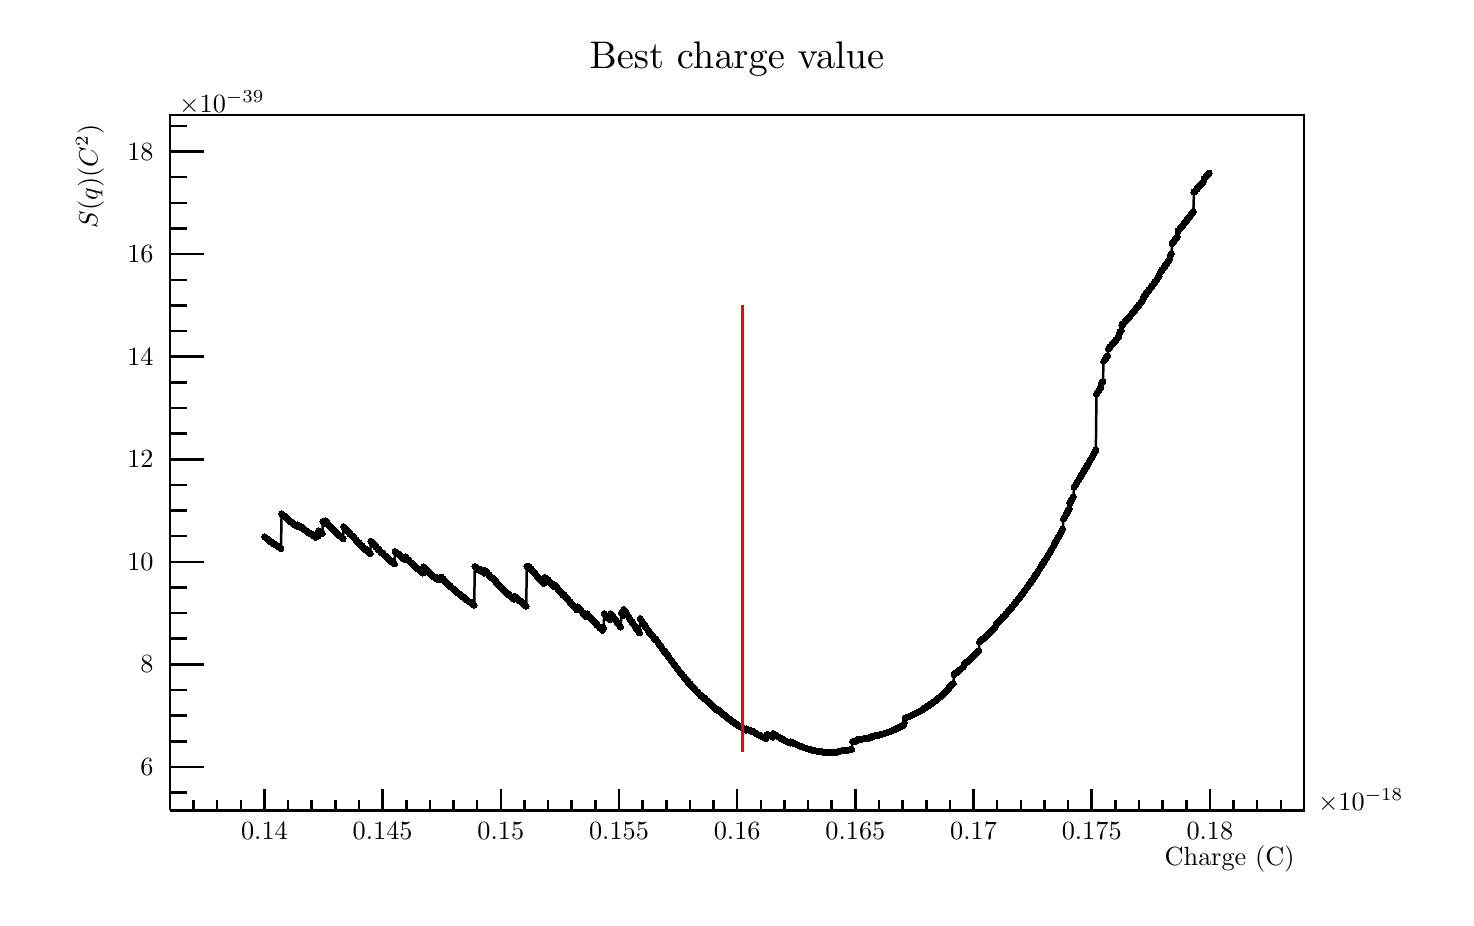
\begin{tikzpicture}[scale=0.90]
\def\CheckTikzLibraryLoaded#1{ \ifcsname tikz@library@#1@loaded\endcsname \else \PackageWarning{tikz}{usetikzlibrary{#1} is missing in the preamble.} \fi }
\CheckTikzLibraryLoaded{patterns}
\CheckTikzLibraryLoaded{plotmarks}
\pgfdeclareplotmark{cross} {
\pgfpathmoveto{\pgfpoint{-0.3\pgfplotmarksize}{\pgfplotmarksize}}
\pgfpathlineto{\pgfpoint{+0.3\pgfplotmarksize}{\pgfplotmarksize}}
\pgfpathlineto{\pgfpoint{+0.3\pgfplotmarksize}{0.3\pgfplotmarksize}}
\pgfpathlineto{\pgfpoint{+1\pgfplotmarksize}{0.3\pgfplotmarksize}}
\pgfpathlineto{\pgfpoint{+1\pgfplotmarksize}{-0.3\pgfplotmarksize}}
\pgfpathlineto{\pgfpoint{+0.3\pgfplotmarksize}{-0.3\pgfplotmarksize}}
\pgfpathlineto{\pgfpoint{+0.3\pgfplotmarksize}{-1.\pgfplotmarksize}}
\pgfpathlineto{\pgfpoint{-0.3\pgfplotmarksize}{-1.\pgfplotmarksize}}
\pgfpathlineto{\pgfpoint{-0.3\pgfplotmarksize}{-0.3\pgfplotmarksize}}
\pgfpathlineto{\pgfpoint{-1.\pgfplotmarksize}{-0.3\pgfplotmarksize}}
\pgfpathlineto{\pgfpoint{-1.\pgfplotmarksize}{0.3\pgfplotmarksize}}
\pgfpathlineto{\pgfpoint{-0.3\pgfplotmarksize}{0.3\pgfplotmarksize}}
\pgfpathclose
\pgfusepathqstroke
}
\pgfdeclareplotmark{cross*} {
\pgfpathmoveto{\pgfpoint{-0.3\pgfplotmarksize}{\pgfplotmarksize}}
\pgfpathlineto{\pgfpoint{+0.3\pgfplotmarksize}{\pgfplotmarksize}}
\pgfpathlineto{\pgfpoint{+0.3\pgfplotmarksize}{0.3\pgfplotmarksize}}
\pgfpathlineto{\pgfpoint{+1\pgfplotmarksize}{0.3\pgfplotmarksize}}
\pgfpathlineto{\pgfpoint{+1\pgfplotmarksize}{-0.3\pgfplotmarksize}}
\pgfpathlineto{\pgfpoint{+0.3\pgfplotmarksize}{-0.3\pgfplotmarksize}}
\pgfpathlineto{\pgfpoint{+0.3\pgfplotmarksize}{-1.\pgfplotmarksize}}
\pgfpathlineto{\pgfpoint{-0.3\pgfplotmarksize}{-1.\pgfplotmarksize}}
\pgfpathlineto{\pgfpoint{-0.3\pgfplotmarksize}{-0.3\pgfplotmarksize}}
\pgfpathlineto{\pgfpoint{-1.\pgfplotmarksize}{-0.3\pgfplotmarksize}}
\pgfpathlineto{\pgfpoint{-1.\pgfplotmarksize}{0.3\pgfplotmarksize}}
\pgfpathlineto{\pgfpoint{-0.3\pgfplotmarksize}{0.3\pgfplotmarksize}}
\pgfpathclose
\pgfusepathqfillstroke
}
\pgfdeclareplotmark{newstar} {
\pgfpathmoveto{\pgfqpoint{0pt}{\pgfplotmarksize}}
\pgfpathlineto{\pgfqpointpolar{44}{0.5\pgfplotmarksize}}
\pgfpathlineto{\pgfqpointpolar{18}{\pgfplotmarksize}}
\pgfpathlineto{\pgfqpointpolar{-20}{0.5\pgfplotmarksize}}
\pgfpathlineto{\pgfqpointpolar{-54}{\pgfplotmarksize}}
\pgfpathlineto{\pgfqpointpolar{-90}{0.5\pgfplotmarksize}}
\pgfpathlineto{\pgfqpointpolar{234}{\pgfplotmarksize}}
\pgfpathlineto{\pgfqpointpolar{198}{0.5\pgfplotmarksize}}
\pgfpathlineto{\pgfqpointpolar{162}{\pgfplotmarksize}}
\pgfpathlineto{\pgfqpointpolar{134}{0.5\pgfplotmarksize}}
\pgfpathclose
\pgfusepathqstroke
}
\pgfdeclareplotmark{newstar*} {
\pgfpathmoveto{\pgfqpoint{0pt}{\pgfplotmarksize}}
\pgfpathlineto{\pgfqpointpolar{44}{0.5\pgfplotmarksize}}
\pgfpathlineto{\pgfqpointpolar{18}{\pgfplotmarksize}}
\pgfpathlineto{\pgfqpointpolar{-20}{0.5\pgfplotmarksize}}
\pgfpathlineto{\pgfqpointpolar{-54}{\pgfplotmarksize}}
\pgfpathlineto{\pgfqpointpolar{-90}{0.5\pgfplotmarksize}}
\pgfpathlineto{\pgfqpointpolar{234}{\pgfplotmarksize}}
\pgfpathlineto{\pgfqpointpolar{198}{0.5\pgfplotmarksize}}
\pgfpathlineto{\pgfqpointpolar{162}{\pgfplotmarksize}}
\pgfpathlineto{\pgfqpointpolar{134}{0.5\pgfplotmarksize}}
\pgfpathclose
\pgfusepathqfillstroke
}
\definecolor{c}{rgb}{1,1,1};
\draw [color=c, fill=c] (0,0) rectangle (20,12.2628);
\draw [color=c, fill=c] (2,1.22628) rectangle (18,11.0365);
\definecolor{c}{rgb}{0,0,0};
\draw [c,line width=0.9] (2,1.22628) -- (2,11.0365) -- (18,11.0365) -- (18,1.22628) -- (2,1.22628);
\definecolor{c}{rgb}{1,1,1};
\draw [color=c, fill=c] (2,1.22628) rectangle (18,11.0365);
\definecolor{c}{rgb}{0,0,0};
\draw [c,line width=0.9] (2,1.22628) -- (2,11.0365) -- (18,11.0365) -- (18,1.22628) -- (2,1.22628);
\draw [c,line width=0.9] (2,1.22628) -- (18,1.22628);
\draw [c,line width=0.9] (3.33333,1.52058) -- (3.33333,1.22628);
\draw [c,line width=0.9] (3.66688,1.37343) -- (3.66688,1.22628);
\draw [c,line width=0.9] (4.00042,1.37343) -- (4.00042,1.22628);
\draw [c,line width=0.9] (4.33396,1.37343) -- (4.33396,1.22628);
\draw [c,line width=0.9] (4.6675,1.37343) -- (4.6675,1.22628);
\draw [c,line width=0.9] (5.00104,1.52058) -- (5.00104,1.22628);
\draw [c,line width=0.9] (5.33458,1.37343) -- (5.33458,1.22628);
\draw [c,line width=0.9] (5.66813,1.37343) -- (5.66813,1.22628);
\draw [c,line width=0.9] (6.00167,1.37343) -- (6.00167,1.22628);
\draw [c,line width=0.9] (6.33521,1.37343) -- (6.33521,1.22628);
\draw [c,line width=0.9] (6.66875,1.52058) -- (6.66875,1.22628);
\draw [c,line width=0.9] (7.00229,1.37343) -- (7.00229,1.22628);
\draw [c,line width=0.9] (7.33583,1.37343) -- (7.33583,1.22628);
\draw [c,line width=0.9] (7.66938,1.37343) -- (7.66938,1.22628);
\draw [c,line width=0.9] (8.00292,1.37343) -- (8.00292,1.22628);
\draw [c,line width=0.9] (8.33646,1.52058) -- (8.33646,1.22628);
\draw [c,line width=0.9] (8.67,1.37343) -- (8.67,1.22628);
\draw [c,line width=0.9] (9.00354,1.37343) -- (9.00354,1.22628);
\draw [c,line width=0.9] (9.33709,1.37343) -- (9.33709,1.22628);
\draw [c,line width=0.9] (9.67063,1.37343) -- (9.67063,1.22628);
\draw [c,line width=0.9] (10.0042,1.52058) -- (10.0042,1.22628);
\draw [c,line width=0.9] (10.3377,1.37343) -- (10.3377,1.22628);
\draw [c,line width=0.9] (10.6713,1.37343) -- (10.6713,1.22628);
\draw [c,line width=0.9] (11.0048,1.37343) -- (11.0048,1.22628);
\draw [c,line width=0.9] (11.3383,1.37343) -- (11.3383,1.22628);
\draw [c,line width=0.9] (11.6719,1.52058) -- (11.6719,1.22628);
\draw [c,line width=0.9] (12.0054,1.37343) -- (12.0054,1.22628);
\draw [c,line width=0.9] (12.339,1.37343) -- (12.339,1.22628);
\draw [c,line width=0.9] (12.6725,1.37343) -- (12.6725,1.22628);
\draw [c,line width=0.9] (13.006,1.37343) -- (13.006,1.22628);
\draw [c,line width=0.9] (13.3396,1.52058) -- (13.3396,1.22628);
\draw [c,line width=0.9] (13.6731,1.37343) -- (13.6731,1.22628);
\draw [c,line width=0.9] (14.0067,1.37343) -- (14.0067,1.22628);
\draw [c,line width=0.9] (14.3402,1.37343) -- (14.3402,1.22628);
\draw [c,line width=0.9] (14.6738,1.37343) -- (14.6738,1.22628);
\draw [c,line width=0.9] (15.0073,1.52058) -- (15.0073,1.22628);
\draw [c,line width=0.9] (15.3408,1.37343) -- (15.3408,1.22628);
\draw [c,line width=0.9] (15.6744,1.37343) -- (15.6744,1.22628);
\draw [c,line width=0.9] (16.0079,1.37343) -- (16.0079,1.22628);
\draw [c,line width=0.9] (16.3415,1.37343) -- (16.3415,1.22628);
\draw [c,line width=0.9] (16.675,1.52058) -- (16.675,1.22628);
\draw [c,line width=0.9] (3.33333,1.52058) -- (3.33333,1.22628);
\draw [c,line width=0.9] (2.99979,1.37343) -- (2.99979,1.22628);
\draw [c,line width=0.9] (2.66625,1.37343) -- (2.66625,1.22628);
\draw [c,line width=0.9] (2.33271,1.37343) -- (2.33271,1.22628);
\draw [c,line width=0.9] (16.675,1.52058) -- (16.675,1.22628);
\draw [c,line width=0.9] (17.0085,1.37343) -- (17.0085,1.22628);
\draw [c,line width=0.9] (17.3421,1.37343) -- (17.3421,1.22628);
\draw [c,line width=0.9] (17.6756,1.37343) -- (17.6756,1.22628);
\draw [anchor=base] (3.33333,0.821606) node[scale=0.949528, color=c, rotate=0]{0.14};
\draw [anchor=base] (5.00104,0.821606) node[scale=0.949528, color=c, rotate=0]{0.145};
\draw [anchor=base] (6.66875,0.821606) node[scale=0.949528, color=c, rotate=0]{0.15};
\draw [anchor=base] (8.33646,0.821606) node[scale=0.949528, color=c, rotate=0]{0.155};
\draw [anchor=base] (10.0042,0.821606) node[scale=0.949528, color=c, rotate=0]{0.16};
\draw [anchor=base] (11.6719,0.821606) node[scale=0.949528, color=c, rotate=0]{0.165};
\draw [anchor=base] (13.3396,0.821606) node[scale=0.949528, color=c, rotate=0]{0.17};
\draw [anchor=base] (15.0073,0.821606) node[scale=0.949528, color=c, rotate=0]{0.175};
\draw [anchor=base] (16.675,0.821606) node[scale=0.949528, color=c, rotate=0]{0.18};
\draw [anchor=base west] (18.07,1.22628) node[scale=0.949528, color=c, rotate=0]{$\times10^{-18}$};
\draw [anchor= east] (18,0.539562) node[scale=0.949528, color=c, rotate=0]{Charge (C)};
\draw [c,line width=0.9] (2,1.22628) -- (2,11.0365);
\draw [c,line width=0.9] (2.48,1.83848) -- (2,1.83848);
\draw [c,line width=0.9] (2.24,2.20031) -- (2,2.20031);
\draw [c,line width=0.9] (2.24,2.56214) -- (2,2.56214);
\draw [c,line width=0.9] (2.24,2.92396) -- (2,2.92396);
\draw [c,line width=0.9] (2.48,3.28579) -- (2,3.28579);
\draw [c,line width=0.9] (2.24,3.64762) -- (2,3.64762);
\draw [c,line width=0.9] (2.24,4.00944) -- (2,4.00944);
\draw [c,line width=0.9] (2.24,4.37127) -- (2,4.37127);
\draw [c,line width=0.9] (2.48,4.7331) -- (2,4.7331);
\draw [c,line width=0.9] (2.24,5.09492) -- (2,5.09492);
\draw [c,line width=0.9] (2.24,5.45675) -- (2,5.45675);
\draw [c,line width=0.9] (2.24,5.81858) -- (2,5.81858);
\draw [c,line width=0.9] (2.48,6.1804) -- (2,6.1804);
\draw [c,line width=0.9] (2.24,6.54223) -- (2,6.54223);
\draw [c,line width=0.9] (2.24,6.90406) -- (2,6.90406);
\draw [c,line width=0.9] (2.24,7.26588) -- (2,7.26588);
\draw [c,line width=0.9] (2.48,7.62771) -- (2,7.62771);
\draw [c,line width=0.9] (2.24,7.98954) -- (2,7.98954);
\draw [c,line width=0.9] (2.24,8.35136) -- (2,8.35136);
\draw [c,line width=0.9] (2.24,8.71319) -- (2,8.71319);
\draw [c,line width=0.9] (2.48,9.07502) -- (2,9.07502);
\draw [c,line width=0.9] (2.24,9.43684) -- (2,9.43684);
\draw [c,line width=0.9] (2.24,9.79867) -- (2,9.79867);
\draw [c,line width=0.9] (2.24,10.1605) -- (2,10.1605);
\draw [c,line width=0.9] (2.48,10.5223) -- (2,10.5223);
\draw [c,line width=0.9] (2.48,1.83848) -- (2,1.83848);
\draw [c,line width=0.9] (2.24,1.47666) -- (2,1.47666);
\draw [c,line width=0.9] (2.48,10.5223) -- (2,10.5223);
\draw [c,line width=0.9] (2.24,10.8841) -- (2,10.8841);
\draw [anchor= east] (1.9,1.83848) node[scale=0.949528, color=c, rotate=0]{6};
\draw [anchor= east] (1.9,3.28579) node[scale=0.949528, color=c, rotate=0]{8};
\draw [anchor= east] (1.9,4.7331) node[scale=0.949528, color=c, rotate=0]{10};
\draw [anchor= east] (1.9,6.1804) node[scale=0.949528, color=c, rotate=0]{12};
\draw [anchor= east] (1.9,7.62771) node[scale=0.949528, color=c, rotate=0]{14};
\draw [anchor= east] (1.9,9.07502) node[scale=0.949528, color=c, rotate=0]{16};
\draw [anchor= east] (1.9,10.5223) node[scale=0.949528, color=c, rotate=0]{18};
\draw [anchor=base west] (2,11.0794) node[scale=0.949528, color=c, rotate=0]{$\times10^{-39}$};
\draw [anchor= east] (0.872471,11.0365) node[scale=0.949528, color=c, rotate=90]{$S(q) (C^{2})$};
\draw [c,line width=0.9] (3.33333,5.08815) -- (3.34167,5.08117) -- (3.35001,5.07426) -- (3.35835,5.06742) -- (3.36669,5.06064) -- (3.37503,5.05393) -- (3.38336,5.04728) -- (3.3917,5.04071) -- (3.40004,5.0342) -- (3.40838,5.02775) -- (3.41672,5.02138)
 -- (3.42506,5.01507) -- (3.4334,5.00883) -- (3.44173,5.00265) -- (3.45007,4.99654) -- (3.45841,4.9905) -- (3.46675,4.98453) -- (3.47509,4.9869) -- (3.48343,4.98052) -- (3.49177,4.97421) -- (3.5001,4.96797) -- (3.50844,4.96179) -- (3.51678,4.95568)
 -- (3.52512,4.94964) -- (3.53346,4.94367) -- (3.5418,4.93776) -- (3.55014,4.93192) -- (3.55847,4.92614) -- (3.56681,4.92043) -- (3.57515,5.41193) -- (3.58349,5.40424) -- (3.59183,5.39661) -- (3.60017,5.38905) -- (3.60851,5.38155) --
 (3.61684,5.37413) -- (3.62518,5.36677) -- (3.63352,5.35947) -- (3.64186,5.35224) -- (3.6502,5.34508) -- (3.65854,5.33799) -- (3.66688,5.33097) -- (3.67521,5.32401) -- (3.68355,5.31711) -- (3.69189,5.31029) -- (3.70023,5.30353) -- (3.70857,5.29684)
 -- (3.71691,5.29022) -- (3.72524,5.28366) -- (3.73358,5.27717) -- (3.74192,5.27074) -- (3.75026,5.26439) -- (3.7586,5.2581) -- (3.76694,5.25187) -- (3.77528,5.24572) -- (3.78361,5.23963) -- (3.79195,5.23361) -- (3.80029,5.25382) -- (3.80863,5.24714)
 -- (3.81697,5.24052) -- (3.82531,5.23398) -- (3.83365,5.2275) -- (3.84198,5.22109) -- (3.85032,5.22613) -- (3.85866,5.21925) -- (3.867,5.21243) -- (3.87534,5.20568) -- (3.88368,5.199) -- (3.89202,5.19238) -- (3.90035,5.18584) -- (3.90869,5.17935) --
 (3.91703,5.17294) -- (3.92537,5.16659) -- (3.93371,5.16031) -- (3.94205,5.1541) -- (3.95039,5.14795) -- (3.95872,5.14187) -- (3.96706,5.14429) -- (3.9754,5.1378) -- (3.98374,5.13138) -- (3.99208,5.12503) -- (4.00042,5.11874) -- (4.00876,5.11252) --
 (4.01709,5.10637) -- (4.02543,5.10028) -- (4.03377,5.09427) -- (4.04211,5.08831) -- (4.05045,5.08243) -- (4.05879,5.07661) -- (4.06713,5.11487) -- (4.07546,5.10825) -- (4.0838,5.10169) -- (4.09214,5.09519) -- (4.10048,5.17066) -- (4.10882,5.16315)
 -- (4.11716,5.15569) -- (4.12549,5.14831) -- (4.13383,5.14099) -- (4.14217,5.14226) -- (4.15051,5.13454) -- (4.15885,5.30428) -- (4.16719,5.29518) -- (4.17553,5.28615) -- (4.18387,5.27719) -- (4.1922,5.3128) -- (4.20054,5.30303) -- (4.20888,5.29332)
 -- (4.21722,5.28368) -- (4.22556,5.2741) -- (4.2339,5.2646) -- (4.24223,5.25516) -- (4.25057,5.24578) -- (4.25891,5.23648) -- (4.26725,5.22724) -- (4.27559,5.21807) -- (4.28393,5.20896) -- (4.29227,5.19992) -- (4.3006,5.19095) -- (4.30894,5.18205)
 -- (4.31728,5.17321) -- (4.32562,5.16444) -- (4.33396,5.15573) -- (4.3423,5.1471) -- (4.35064,5.13853) -- (4.35897,5.13002) -- (4.36731,5.12159) -- (4.37565,5.11322) -- (4.38399,5.10492) -- (4.39233,5.09668) -- (4.40067,5.1001) -- (4.40901,5.09139)
 -- (4.41734,5.08274) -- (4.42568,5.07416) -- (4.43402,5.06565) -- (4.44236,5.05721) -- (4.4507,5.22909) -- (4.45904,5.21927) -- (4.46738,5.20951) -- (4.47571,5.19982) -- (4.48405,5.1902) -- (4.49239,5.18064) -- (4.50073,5.17115) -- (4.50907,5.16173)
 -- (4.51741,5.15238) -- (4.52575,5.14309) -- (4.53408,5.13387) -- (4.54242,5.12471) -- (4.55076,5.11562) -- (4.5591,5.1066) -- (4.56744,5.10606) -- (4.57578,5.09663) -- (4.58412,5.08726) -- (4.59245,5.07796) -- (4.60079,5.06872) -- (4.60913,5.05956)
 -- (4.61747,5.05045) -- (4.62581,5.04142) -- (4.63415,5.03245) -- (4.64249,5.02355) -- (4.65082,5.01472) -- (4.65916,5.00595) -- (4.6675,4.99725) -- (4.67584,4.98862) -- (4.68418,4.98006) -- (4.69252,4.97156) -- (4.70085,4.96313) --
 (4.70919,4.95476) -- (4.71753,4.94646) -- (4.72587,4.93823) -- (4.73421,4.93007) -- (4.74255,4.92197) -- (4.75089,4.91394) -- (4.75922,4.90598) -- (4.76756,4.89808) -- (4.7759,4.89889) -- (4.78424,4.89058) -- (4.79258,4.88233) -- (4.80092,4.87415)
 -- (4.80926,4.86604) -- (4.81759,4.85799) -- (4.82593,4.85001) -- (4.83427,5.02482) -- (4.84261,5.01545) -- (4.85095,5.00615) -- (4.85929,4.99691) -- (4.86763,4.98775) -- (4.87596,4.97864) -- (4.8843,4.96961) -- (4.89264,4.96064) --
 (4.90098,4.95174) -- (4.90932,4.94291) -- (4.91766,4.93414) -- (4.926,4.92544) -- (4.93433,4.91681) -- (4.94267,4.90824) -- (4.95101,4.89974) -- (4.95935,4.89131) -- (4.96769,4.88294) -- (4.97603,4.87464) -- (4.98437,4.86641) -- (4.9927,4.85825) --
 (5.00104,4.85015) -- (5.00938,4.84212) -- (5.01772,4.83415) -- (5.02606,4.82626) -- (5.0344,4.81843) -- (5.04274,4.81066) -- (5.05107,4.80297) -- (5.05941,4.79534) -- (5.06775,4.78778) -- (5.07609,4.78028) -- (5.08443,4.77285) -- (5.09277,4.76549)
 -- (5.1011,4.7582) -- (5.10944,4.75097) -- (5.11778,4.74381) -- (5.12612,4.73671) -- (5.13446,4.72969) -- (5.1428,4.72273) -- (5.15114,4.71583) -- (5.15947,4.70901) -- (5.16781,4.70225) -- (5.17615,4.88112) -- (5.18449,4.87295) -- (5.19283,4.86486)
 -- (5.20117,4.85683) -- (5.20951,4.84887) -- (5.21784,4.85349) -- (5.22618,4.84504) -- (5.23452,4.83666) -- (5.24286,4.82835) -- (5.2512,4.8201) -- (5.25954,4.81192) -- (5.26788,4.80381) -- (5.27621,4.79576) -- (5.28455,4.78778) -- (5.29289,4.77987)
 -- (5.30123,4.77202) -- (5.30957,4.76424) -- (5.31791,4.80345) -- (5.32625,4.79484) -- (5.33458,4.78629) -- (5.34292,4.77781) -- (5.35126,4.7694) -- (5.3596,4.76106) -- (5.36794,4.75278) -- (5.37628,4.74457) -- (5.38462,4.73642) -- (5.39295,4.72834)
 -- (5.40129,4.72033) -- (5.40963,4.71239) -- (5.41797,4.70451) -- (5.42631,4.6967) -- (5.43465,4.68896) -- (5.44299,4.68128) -- (5.45132,4.67368) -- (5.45966,4.66613) -- (5.468,4.65866) -- (5.47634,4.65125) -- (5.48468,4.64391) -- (5.49302,4.63663)
 -- (5.50136,4.62943) -- (5.50969,4.62229) -- (5.51803,4.61521) -- (5.52637,4.60821) -- (5.53471,4.60127) -- (5.54305,4.59439) -- (5.55139,4.58759) -- (5.55972,4.58085) -- (5.56806,4.57418) -- (5.5764,4.66152) -- (5.58474,4.65303) --
 (5.59308,4.64462) -- (5.60142,4.63626) -- (5.60976,4.62798) -- (5.61809,4.61976) -- (5.62643,4.61161) -- (5.63477,4.60353) -- (5.64311,4.59552) -- (5.65145,4.58757) -- (5.65979,4.57969) -- (5.66813,4.57187) -- (5.67646,4.56412) -- (5.6848,4.55644)
 -- (5.69314,4.54883) -- (5.70148,4.54128) -- (5.70982,4.5338) -- (5.71816,4.52639) -- (5.7265,4.51904) -- (5.73483,4.51176) -- (5.74317,4.50455) -- (5.75151,4.4974) -- (5.75985,4.49032) -- (5.76819,4.51198) -- (5.77653,4.50421) -- (5.78487,4.49651)
 -- (5.7932,4.48887) -- (5.80154,4.4813) -- (5.80988,4.48636) -- (5.81822,4.4783) -- (5.82656,4.5183) -- (5.8349,4.50939) -- (5.84324,4.50055) -- (5.85157,4.49177) -- (5.85991,4.48306) -- (5.86825,4.47442) -- (5.87659,4.46585) -- (5.88493,4.45734) --
 (5.89327,4.4489) -- (5.90161,4.44053) -- (5.90994,4.43222) -- (5.91828,4.42398) -- (5.92662,4.41581) -- (5.93496,4.4077) -- (5.9433,4.39966) -- (5.95164,4.39169) -- (5.95998,4.38379) -- (5.96831,4.37595) -- (5.97665,4.36818) -- (5.98499,4.36047) --
 (5.99333,4.35284) -- (6.00167,4.34527) -- (6.01001,4.33776) -- (6.01834,4.33033) -- (6.02668,4.32296) -- (6.03502,4.31565) -- (6.04336,4.30842) -- (6.0517,4.30125) -- (6.06004,4.29415) -- (6.06838,4.28711) -- (6.07671,4.28914) -- (6.08505,4.28167)
 -- (6.09339,4.27427) -- (6.10173,4.26694) -- (6.11007,4.25967) -- (6.11841,4.25247) -- (6.12675,4.24534) -- (6.13508,4.23828) -- (6.14342,4.23128) -- (6.15176,4.22435) -- (6.1601,4.21748) -- (6.16844,4.21068) -- (6.17678,4.20395) --
 (6.18512,4.19729) -- (6.19345,4.19069) -- (6.20179,4.18416) -- (6.21013,4.1777) -- (6.21847,4.1713) -- (6.22681,4.17174) -- (6.23515,4.16497) -- (6.24349,4.15826) -- (6.25182,4.15162) -- (6.26016,4.14504) -- (6.2685,4.13854) -- (6.27684,4.13209) --
 (6.28518,4.12572) -- (6.29352,4.11941) -- (6.30186,4.66832) -- (6.31019,4.6599) -- (6.31853,4.65155) -- (6.32687,4.64327) -- (6.33521,4.63505) -- (6.34355,4.6269) -- (6.35189,4.61882) -- (6.36023,4.62357) -- (6.36856,4.61499) -- (6.3769,4.60647) --
 (6.38524,4.62729) -- (6.39358,4.61807) -- (6.40192,4.60891) -- (6.41026,4.59983) -- (6.41859,4.59081) -- (6.42693,4.58185) -- (6.43527,4.57297) -- (6.44361,4.61281) -- (6.45195,4.60307) -- (6.46029,4.5934) -- (6.46863,4.58379) -- (6.47696,4.57425)
 -- (6.4853,4.56477) -- (6.49364,4.55537) -- (6.50198,4.54603) -- (6.51032,4.53675) -- (6.51866,4.52755) -- (6.527,4.51841) -- (6.53533,4.50933) -- (6.54367,4.50033) -- (6.55201,4.5046) -- (6.56035,4.49509) -- (6.56869,4.48565) -- (6.57703,4.47627)
 -- (6.58537,4.46696) -- (6.5937,4.45772) -- (6.60204,4.44854) -- (6.61038,4.43943) -- (6.61872,4.43039) -- (6.62706,4.42141) -- (6.6354,4.4125) -- (6.64374,4.40366) -- (6.65207,4.39489) -- (6.66041,4.38618) -- (6.66875,4.37754) -- (6.67709,4.36896)
 -- (6.68543,4.36046) -- (6.69377,4.35202) -- (6.70211,4.34364) -- (6.71044,4.33534) -- (6.71878,4.3271) -- (6.72712,4.31893) -- (6.73546,4.31082) -- (6.7438,4.30278) -- (6.75214,4.29481) -- (6.76048,4.28691) -- (6.76881,4.27907) -- (6.77715,4.2713)
 -- (6.78549,4.26359) -- (6.79383,4.25596) -- (6.80217,4.24839) -- (6.81051,4.24089) -- (6.81885,4.23345) -- (6.82718,4.22608) -- (6.83552,4.21878) -- (6.84386,4.21154) -- (6.8522,4.20437) -- (6.86054,4.24695) -- (6.86888,4.23891) --
 (6.87721,4.23095) -- (6.88555,4.22305) -- (6.89389,4.21521) -- (6.90223,4.20745) -- (6.91057,4.19975) -- (6.91891,4.19212) -- (6.92725,4.18456) -- (6.93559,4.17706) -- (6.94392,4.18308) -- (6.95226,4.17508) -- (6.9606,4.16714) -- (6.96894,4.15926)
 -- (6.97728,4.15145) -- (6.98562,4.14371) -- (6.99395,4.13604) -- (7.00229,4.12843) -- (7.01063,4.1209) -- (7.01897,4.11342) -- (7.02731,4.10602) -- (7.03565,4.67038) -- (7.04399,4.66083) -- (7.05232,4.65135) -- (7.06066,4.67168) -- (7.069,4.66148)
 -- (7.07734,4.65136) -- (7.08568,4.6413) -- (7.09402,4.6313) -- (7.10236,4.62137) -- (7.11069,4.61151) -- (7.11903,4.60172) -- (7.12737,4.59199) -- (7.13571,4.58233) -- (7.14405,4.57274) -- (7.15239,4.56322) -- (7.16073,4.55376) -- (7.16906,4.54437)
 -- (7.1774,4.53504) -- (7.18574,4.52578) -- (7.19408,4.51659) -- (7.20242,4.50747) -- (7.21076,4.49841) -- (7.2191,4.48942) -- (7.22743,4.4805) -- (7.23577,4.47164) -- (7.24411,4.46285) -- (7.25245,4.45413) -- (7.26079,4.44548) -- (7.26913,4.43689)
 -- (7.27747,4.42837) -- (7.2858,4.51349) -- (7.29414,4.50387) -- (7.30248,4.49431) -- (7.31082,4.48482) -- (7.31916,4.4754) -- (7.3275,4.46604) -- (7.33583,4.47674) -- (7.34417,4.46679) -- (7.35251,4.45689) -- (7.36085,4.44707) -- (7.36919,4.43731)
 -- (7.37753,4.42762) -- (7.38587,4.418) -- (7.3942,4.40844) -- (7.40254,4.39895) -- (7.41088,4.38953) -- (7.41922,4.38017) -- (7.42756,4.41051) -- (7.4359,4.39982) -- (7.44424,4.38918) -- (7.45257,4.37862) -- (7.46091,4.36812) -- (7.46925,4.35769)
 -- (7.47759,4.34733) -- (7.48593,4.33703) -- (7.49427,4.3268) -- (7.50261,4.31664) -- (7.51094,4.30655) -- (7.51928,4.29652) -- (7.52762,4.28655) -- (7.53596,4.27666) -- (7.5443,4.26683) -- (7.55264,4.25707) -- (7.56098,4.2673) -- (7.56931,4.25693)
 -- (7.57765,4.24663) -- (7.58599,4.2364) -- (7.59433,4.22623) -- (7.60267,4.21613) -- (7.61101,4.2061) -- (7.61935,4.19614) -- (7.62768,4.18624) -- (7.63602,4.17641) -- (7.64436,4.16664) -- (7.6527,4.15694) -- (7.66104,4.14731) -- (7.66938,4.13775)
 -- (7.67772,4.12825) -- (7.68605,4.11882) -- (7.69439,4.10946) -- (7.70273,4.10016) -- (7.71107,4.09093) -- (7.71941,4.08177) -- (7.72775,4.07268) -- (7.73608,4.06365) -- (7.74442,4.05469) -- (7.75276,4.09716) -- (7.7611,4.08732) --
 (7.76944,4.07754) -- (7.77778,4.06783) -- (7.78612,4.05819) -- (7.79446,4.04861) -- (7.80279,4.0391) -- (7.81113,4.02966) -- (7.81947,4.02028) -- (7.82781,4.01098) -- (7.83615,4.00173) -- (7.84449,3.99256) -- (7.85282,3.98345) -- (7.86116,3.97441)
 -- (7.8695,3.96544) -- (7.87784,3.95653) -- (7.88618,3.99933) -- (7.89452,3.98954) -- (7.90286,3.97981) -- (7.91119,3.97015) -- (7.91953,3.96056) -- (7.92787,3.95104) -- (7.93621,3.94158) -- (7.94455,3.93219) -- (7.95289,3.92287) --
 (7.96123,3.91361) -- (7.96956,3.90442) -- (7.9779,3.8953) -- (7.98624,3.88624) -- (7.99458,3.87725) -- (8.00292,3.86833) -- (8.01126,3.85948) -- (8.0196,3.85069) -- (8.02793,3.84197) -- (8.03627,3.83331) -- (8.04461,3.82473) -- (8.05295,3.81621) --
 (8.06129,3.80775) -- (8.06963,3.79937) -- (8.07797,3.79105) -- (8.0863,3.78279) -- (8.09464,3.77461) -- (8.10298,3.76649) -- (8.11132,3.81044) -- (8.11966,3.80143) -- (8.128,4.00183) -- (8.13634,3.99133) -- (8.14467,3.98089) -- (8.15301,3.97052) --
 (8.16135,3.96022) -- (8.16969,3.94998) -- (8.17803,3.93981) -- (8.18637,3.94988) -- (8.19471,3.93909) -- (8.20304,3.92838) -- (8.21138,3.91773) -- (8.21972,4.00421) -- (8.22806,3.99244) -- (8.2364,3.98073) -- (8.24474,3.96909) -- (8.25307,3.95751)
 -- (8.26141,3.946) -- (8.26975,3.93456) -- (8.27809,3.92319) -- (8.28643,3.91188) -- (8.29477,3.90065) -- (8.30311,3.88947) -- (8.31144,3.87837) -- (8.31978,3.86733) -- (8.32812,3.85636) -- (8.33646,3.84545) -- (8.3448,3.83461) -- (8.35314,3.82384)
 -- (8.36148,3.81314) -- (8.36981,4.01309) -- (8.37815,4.00088) -- (8.38649,3.98874) -- (8.39483,3.97667) -- (8.40317,4.06271) -- (8.41151,4.0495) -- (8.41985,4.03637) -- (8.42818,4.0233) -- (8.43652,4.0103) -- (8.44486,3.99736) -- (8.4532,3.9845) --
 (8.46154,3.97169) -- (8.46988,3.95896) -- (8.47822,3.94629) -- (8.48655,3.93369) -- (8.49489,3.92116) -- (8.50323,3.90869) -- (8.51157,3.89629) -- (8.51991,3.88396) -- (8.52825,3.8717) -- (8.53659,3.8595) -- (8.54492,3.84737) -- (8.55326,3.8353) --
 (8.5616,3.8233) -- (8.56994,3.81137) -- (8.57828,3.79951) -- (8.58662,3.78771) -- (8.59496,3.77598) -- (8.60329,3.76432) -- (8.61163,3.75272) -- (8.61997,3.74119) -- (8.62831,3.72973) -- (8.63665,3.9311) -- (8.64499,3.91813) -- (8.65333,3.90522) --
 (8.66166,3.89238) -- (8.67,3.87961) -- (8.67834,3.86691) -- (8.68668,3.85427) -- (8.69502,3.8417) -- (8.70336,3.82919) -- (8.71169,3.81675) -- (8.72003,3.80438) -- (8.72837,3.79208) -- (8.73671,3.77984) -- (8.74505,3.76767) -- (8.75339,3.75557) --
 (8.76173,3.74353) -- (8.77006,3.73156) -- (8.7784,3.71966) -- (8.78674,3.70782) -- (8.79508,3.70997) -- (8.80342,3.6976) -- (8.81176,3.6853) -- (8.8201,3.67306) -- (8.82843,3.66089) -- (8.83677,3.64879) -- (8.84511,3.63676) -- (8.85345,3.64549) --
 (8.86179,3.63283) -- (8.87013,3.62023) -- (8.87847,3.60771) -- (8.8868,3.59525) -- (8.89514,3.58286) -- (8.90348,3.57053) -- (8.91182,3.55828) -- (8.92016,3.54609) -- (8.9285,3.53396) -- (8.93684,3.5219) -- (8.94517,3.50991) -- (8.95351,3.49799) --
 (8.96185,3.48613) -- (8.97019,3.47435) -- (8.97853,3.46262) -- (8.98687,3.46534) -- (8.9952,3.45308) -- (9.00354,3.44089) -- (9.01188,3.42877) -- (9.02022,3.41671) -- (9.02856,3.40472) -- (9.0369,3.39279) -- (9.04524,3.38094) -- (9.05358,3.36915) --
 (9.06191,3.35742) -- (9.07025,3.34577) -- (9.07859,3.33418) -- (9.08693,3.32266) -- (9.09527,3.3112) -- (9.10361,3.29981) -- (9.11195,3.28849) -- (9.12028,3.27724) -- (9.12862,3.26605) -- (9.13696,3.25493) -- (9.1453,3.24387) -- (9.15364,3.23289) --
 (9.16198,3.22197) -- (9.17031,3.21111) -- (9.17865,3.20033) -- (9.18699,3.18961) -- (9.19533,3.17895) -- (9.20367,3.16837) -- (9.21201,3.15785) -- (9.22035,3.1474) -- (9.22868,3.13701) -- (9.23702,3.1267) -- (9.24536,3.11645) -- (9.2537,3.10626) --
 (9.26204,3.09615) -- (9.27038,3.0861) -- (9.27872,3.07611) -- (9.28705,3.0662) -- (9.29539,3.05635) -- (9.30373,3.04657) -- (9.31207,3.03685) -- (9.32041,3.0272) -- (9.32875,3.01762) -- (9.33709,3.00811) -- (9.34542,2.99866) -- (9.35376,2.98928) --
 (9.3621,2.97997) -- (9.37044,2.97072) -- (9.37878,2.96154) -- (9.38712,2.95243) -- (9.39546,2.94338) -- (9.40379,2.9344) -- (9.41213,2.92549) -- (9.42047,2.91664) -- (9.42881,2.90787) -- (9.43715,2.89916) -- (9.44549,2.89051) -- (9.45382,2.88193) --
 (9.46216,2.87342) -- (9.4705,2.86498) -- (9.47884,2.8566) -- (9.48718,2.84829) -- (9.49552,2.84005) -- (9.50386,2.83188) -- (9.5122,2.82377) -- (9.52053,2.81573) -- (9.52887,2.80775) -- (9.53721,2.81445) -- (9.54555,2.80593) -- (9.55389,2.79748) --
 (9.56223,2.78909) -- (9.57057,2.78077) -- (9.5789,2.77252) -- (9.58724,2.76434) -- (9.59558,2.75622) -- (9.60392,2.74817) -- (9.61226,2.74019) -- (9.6206,2.73227) -- (9.62893,2.72443) -- (9.63727,2.71664) -- (9.64561,2.70893) -- (9.65395,2.70128) --
 (9.66229,2.6937) -- (9.67063,2.68618) -- (9.67897,2.67874) -- (9.6873,2.67136) -- (9.69564,2.66404) -- (9.70398,2.6568) -- (9.71232,2.64962) -- (9.72066,2.6425) -- (9.729,2.63546) -- (9.73734,2.64287) -- (9.74567,2.63528) -- (9.75401,2.62776) --
 (9.76235,2.6203) -- (9.77069,2.61291) -- (9.77903,2.60558) -- (9.78737,2.59833) -- (9.79571,2.59114) -- (9.80404,2.58401) -- (9.81238,2.57696) -- (9.82072,2.56997) -- (9.82906,2.56304) -- (9.8374,2.55619) -- (9.84574,2.5494) -- (9.85408,2.54268) --
 (9.86241,2.53602) -- (9.87075,2.52944) -- (9.87909,2.52292) -- (9.88743,2.51646) -- (9.89577,2.51007) -- (9.90411,2.50375) -- (9.91245,2.4975) -- (9.92078,2.49132) -- (9.92912,2.4852) -- (9.93746,2.47914) -- (9.9458,2.47316) -- (9.95414,2.46724) --
 (9.96248,2.46139) -- (9.97081,2.4556) -- (9.97915,2.44989) -- (9.98749,2.44424) -- (9.99583,2.43865) -- (10.0042,2.43314) -- (10.0125,2.42769) -- (10.0208,2.4223) -- (10.0292,2.41699) -- (10.0375,2.41174) -- (10.0459,2.40656) -- (10.0542,2.40144) --
 (10.0625,2.39639) -- (10.0709,2.39141) -- (10.0792,2.3865) -- (10.0876,2.38165) -- (10.0959,2.37687) -- (10.1042,2.37216) -- (10.1126,2.36751) -- (10.1209,2.36293) -- (10.1292,2.35842) -- (10.1376,2.37624) -- (10.1459,2.37108) -- (10.1543,2.36599)
 -- (10.1626,2.36097) -- (10.1709,2.35601) -- (10.1793,2.35113) -- (10.1876,2.3463) -- (10.196,2.34155) -- (10.2043,2.35184) -- (10.2126,2.34653) -- (10.221,2.34129) -- (10.2293,2.33612) -- (10.2376,2.33102) -- (10.246,2.32598) -- (10.2543,2.321) --
 (10.2627,2.3161) -- (10.271,2.31126) -- (10.2793,2.30649) -- (10.2877,2.30179) -- (10.296,2.29715) -- (10.3044,2.29258) -- (10.3127,2.28808) -- (10.321,2.28364) -- (10.3294,2.27927) -- (10.3377,2.27497) -- (10.346,2.27073) -- (10.3544,2.26656) --
 (10.3627,2.26246) -- (10.3711,2.25843) -- (10.3794,2.25446) -- (10.3877,2.25056) -- (10.3961,2.24673) -- (10.4044,2.24296) -- (10.4128,2.23926) -- (10.4211,2.29253) -- (10.4294,2.28789) -- (10.4378,2.29859) -- (10.4461,2.2934) -- (10.4545,2.28828)
 -- (10.4628,2.28322) -- (10.4711,2.27823) -- (10.4795,2.27331) -- (10.4878,2.26845) -- (10.4961,2.26366) -- (10.5045,2.25894) -- (10.5128,2.31128) -- (10.5212,2.30562) -- (10.5295,2.30003) -- (10.5378,2.29451) -- (10.5462,2.28905) --
 (10.5545,2.28365) -- (10.5629,2.27833) -- (10.5712,2.27307) -- (10.5795,2.26788) -- (10.5879,2.26276) -- (10.5962,2.2577) -- (10.6045,2.25271) -- (10.6129,2.24779) -- (10.6212,2.24293) -- (10.6296,2.23814) -- (10.6379,2.23342) -- (10.6462,2.22876)
 -- (10.6546,2.22417) -- (10.6629,2.21965) -- (10.6713,2.2152) -- (10.6796,2.21081) -- (10.6879,2.20649) -- (10.6963,2.20223) -- (10.7046,2.19805) -- (10.7129,2.19393) -- (10.7213,2.18987) -- (10.7296,2.18589) -- (10.738,2.18197) -- (10.7463,2.17812)
 -- (10.7546,2.17433) -- (10.763,2.19313) -- (10.7713,2.1887) -- (10.7797,2.18432) -- (10.788,2.18002) -- (10.7963,2.17578) -- (10.8047,2.17161) -- (10.813,2.16751) -- (10.8213,2.16347) -- (10.8297,2.1595) -- (10.838,2.1556) -- (10.8464,2.15177) --
 (10.8547,2.148) -- (10.863,2.1443) -- (10.8714,2.14066) -- (10.8797,2.13709) -- (10.8881,2.13359) -- (10.8964,2.13016) -- (10.9047,2.12679) -- (10.9131,2.12349) -- (10.9214,2.12026) -- (10.9297,2.11709) -- (10.9381,2.114) -- (10.9464,2.11096) --
 (10.9548,2.108) -- (10.9631,2.1051) -- (10.9714,2.10227) -- (10.9798,2.0995) -- (10.9881,2.09681) -- (10.9965,2.09418) -- (11.0048,2.09161) -- (11.0131,2.08912) -- (11.0215,2.08669) -- (11.0298,2.08432) -- (11.0381,2.08203) -- (11.0465,2.0798) --
 (11.0548,2.07764) -- (11.0632,2.07554) -- (11.0715,2.07351) -- (11.0798,2.07155) -- (11.0882,2.06966) -- (11.0965,2.06783) -- (11.1049,2.06607) -- (11.1132,2.06438) -- (11.1215,2.06275) -- (11.1299,2.06119) -- (11.1382,2.0597) -- (11.1466,2.05827)
 -- (11.1549,2.05691) -- (11.1632,2.05562) -- (11.1716,2.0544) -- (11.1799,2.05324) -- (11.1882,2.05215) -- (11.1966,2.05112) -- (11.2049,2.05017) -- (11.2133,2.04928) -- (11.2216,2.04845) -- (11.2299,2.0477) -- (11.2383,2.04701) -- (11.2466,2.04639)
 -- (11.255,2.04583) -- (11.2633,2.04534) -- (11.2716,2.04492) -- (11.28,2.04456) -- (11.2883,2.04428) -- (11.2966,2.04406) -- (11.305,2.0439) -- (11.3133,2.04382) -- (11.3217,2.0438) -- (11.33,2.04384) -- (11.3383,2.04396) -- (11.3467,2.04414) --
 (11.355,2.04439) -- (11.3634,2.0447) -- (11.3717,2.04508) -- (11.38,2.04553) -- (11.3884,2.04605) -- (11.3967,2.04663) -- (11.405,2.04728) -- (11.4134,2.04799) -- (11.4217,2.04878) -- (11.4301,2.04963) -- (11.4384,2.05054) -- (11.4467,2.06276) --
 (11.4551,2.06318) -- (11.4634,2.06367) -- (11.4718,2.06423) -- (11.4801,2.06485) -- (11.4884,2.06554) -- (11.4968,2.0663) -- (11.5051,2.06713) -- (11.5134,2.06802) -- (11.5218,2.06898) -- (11.5301,2.07) -- (11.5385,2.07109) -- (11.5468,2.07225) --
 (11.5551,2.07348) -- (11.5635,2.07477) -- (11.5718,2.07614) -- (11.5802,2.07756) -- (11.5885,2.07906) -- (11.5968,2.08062) -- (11.6052,2.08225) -- (11.6135,2.08394) -- (11.6218,2.0857) -- (11.6302,2.19773) -- (11.6385,2.19828) -- (11.6469,2.1989) --
 (11.6552,2.19959) -- (11.6635,2.20035) -- (11.6719,2.20117) -- (11.6802,2.20206) -- (11.6886,2.20301) -- (11.6969,2.22734) -- (11.7052,2.22763) -- (11.7136,2.22799) -- (11.7219,2.22841) -- (11.7302,2.2289) -- (11.7386,2.22946) -- (11.7469,2.23009)
 -- (11.7553,2.23078) -- (11.7636,2.23154) -- (11.7719,2.23236) -- (11.7803,2.23325) -- (11.7886,2.23421) -- (11.797,2.23524) -- (11.8053,2.23633) -- (11.8136,2.23749) -- (11.822,2.23872) -- (11.8303,2.24001) -- (11.8386,2.24137) -- (11.847,2.2428)
 -- (11.8553,2.24429) -- (11.8637,2.24585) -- (11.872,2.24748) -- (11.8803,2.24918) -- (11.8887,2.26713) -- (11.897,2.26826) -- (11.9054,2.26944) -- (11.9137,2.2707) -- (11.922,2.27202) -- (11.9304,2.27341) -- (11.9387,2.27487) -- (11.9471,2.27639)
 -- (11.9554,2.27798) -- (11.9637,2.27964) -- (11.9721,2.28136) -- (11.9804,2.28315) -- (11.9887,2.28501) -- (11.9971,2.28694) -- (12.0054,2.28893) -- (12.0138,2.29099) -- (12.0221,2.29311) -- (12.0304,2.2953) -- (12.0388,2.29756) --
 (12.0471,2.29989) -- (12.0555,2.30228) -- (12.0638,2.30474) -- (12.0721,2.30727) -- (12.0805,2.30986) -- (12.0888,2.31253) -- (12.0971,2.31525) -- (12.1055,2.31805) -- (12.1138,2.32091) -- (12.1222,2.32384) -- (12.1305,2.32684) -- (12.1388,2.3299)
 -- (12.1472,2.33303) -- (12.1555,2.33622) -- (12.1639,2.33949) -- (12.1722,2.34282) -- (12.1805,2.34622) -- (12.1889,2.34968) -- (12.1972,2.35321) -- (12.2055,2.35681) -- (12.2139,2.36047) -- (12.2222,2.36421) -- (12.2306,2.36801) --
 (12.2389,2.37187) -- (12.2472,2.3758) -- (12.2556,2.3798) -- (12.2639,2.38387) -- (12.2723,2.388) -- (12.2806,2.39221) -- (12.2889,2.39647) -- (12.2973,2.40081) -- (12.3056,2.40521) -- (12.3139,2.40968) -- (12.3223,2.41421) -- (12.3306,2.41882) --
 (12.339,2.42348) -- (12.3473,2.42822) -- (12.3556,2.43302) -- (12.364,2.46178) -- (12.3723,2.52724) -- (12.3807,2.53032) -- (12.389,2.53347) -- (12.3973,2.53669) -- (12.4057,2.53998) -- (12.414,2.54333) -- (12.4223,2.54675) -- (12.4307,2.55024) --
 (12.439,2.5538) -- (12.4474,2.55742) -- (12.4557,2.56111) -- (12.464,2.56486) -- (12.4724,2.56868) -- (12.4807,2.57257) -- (12.4891,2.57653) -- (12.4974,2.58055) -- (12.5057,2.58464) -- (12.5141,2.5888) -- (12.5224,2.59302) -- (12.5307,2.59731) --
 (12.5391,2.60167) -- (12.5474,2.6061) -- (12.5558,2.61059) -- (12.5641,2.61515) -- (12.5724,2.61977) -- (12.5808,2.62446) -- (12.5891,2.62922) -- (12.5975,2.63405) -- (12.6058,2.63894) -- (12.6141,2.6439) -- (12.6225,2.64893) -- (12.6308,2.65402) --
 (12.6391,2.65919) -- (12.6475,2.66441) -- (12.6558,2.66971) -- (12.6642,2.67507) -- (12.6725,2.6805) -- (12.6808,2.68599) -- (12.6892,2.69156) -- (12.6975,2.69719) -- (12.7059,2.70288) -- (12.7142,2.70865) -- (12.7225,2.71448) -- (12.7309,2.72037)
 -- (12.7392,2.72634) -- (12.7476,2.73237) -- (12.7559,2.73847) -- (12.7642,2.74463) -- (12.7726,2.75087) -- (12.7809,2.75716) -- (12.7892,2.76353) -- (12.7976,2.76996) -- (12.8059,2.77646) -- (12.8143,2.78303) -- (12.8226,2.78966) --
 (12.8309,2.79636) -- (12.8393,2.80313) -- (12.8476,2.80997) -- (12.856,2.81687) -- (12.8643,2.82384) -- (12.8726,2.83087) -- (12.881,2.83797) -- (12.8893,2.84514) -- (12.8976,2.85238) -- (12.906,2.85968) -- (12.9143,2.86705) -- (12.9227,2.87449) --
 (12.931,2.88199) -- (12.9393,2.88956) -- (12.9477,2.8972) -- (12.956,2.90491) -- (12.9644,2.91268) -- (12.9727,2.92052) -- (12.981,2.92842) -- (12.9894,2.96054) -- (12.9977,2.96776) -- (13.006,2.97505) -- (13.0144,2.98241) -- (13.0227,2.98983) --
 (13.0311,2.99732) -- (13.0394,3.00487) -- (13.0477,3.01249) -- (13.0561,3.02018) -- (13.0644,3.14334) -- (13.0728,3.14979) -- (13.0811,3.1563) -- (13.0894,3.16288) -- (13.0978,3.16953) -- (13.1061,3.17624) -- (13.1144,3.18302) -- (13.1228,3.18987)
 -- (13.1311,3.19678) -- (13.1395,3.20376) -- (13.1478,3.21081) -- (13.1561,3.21793) -- (13.1645,3.22511) -- (13.1728,3.23236) -- (13.1812,3.23968) -- (13.1895,3.24706) -- (13.1978,3.25451) -- (13.2062,3.28692) -- (13.2145,3.29368) --
 (13.2228,3.30051) -- (13.2312,3.3074) -- (13.2395,3.31437) -- (13.2479,3.3214) -- (13.2562,3.32849) -- (13.2645,3.33566) -- (13.2729,3.34289) -- (13.2812,3.35019) -- (13.2896,3.35755) -- (13.2979,3.36498) -- (13.3062,3.37248) -- (13.3146,3.38005) --
 (13.3229,3.38768) -- (13.3312,3.39538) -- (13.3396,3.40314) -- (13.3479,3.41098) -- (13.3563,3.41888) -- (13.3646,3.42684) -- (13.3729,3.43488) -- (13.3813,3.44298) -- (13.3896,3.45115) -- (13.398,3.45938) -- (13.4063,3.46768) -- (13.4146,3.47605)
 -- (13.423,3.60216) -- (13.4313,3.60927) -- (13.4396,3.61646) -- (13.448,3.62371) -- (13.4563,3.63102) -- (13.4647,3.63841) -- (13.473,3.64586) -- (13.4813,3.65338) -- (13.4897,3.66096) -- (13.498,3.66862) -- (13.5064,3.67633) -- (13.5147,3.68412)
 -- (13.523,3.69197) -- (13.5314,3.69989) -- (13.5397,3.70788) -- (13.5481,3.71593) -- (13.5564,3.72405) -- (13.5647,3.73224) -- (13.5731,3.7405) -- (13.5814,3.74882) -- (13.5897,3.75721) -- (13.5981,3.76566) -- (13.6064,3.77418) -- (13.6148,3.78277)
 -- (13.6231,3.79143) -- (13.6314,3.80015) -- (13.6398,3.80894) -- (13.6481,3.8178) -- (13.6565,3.85145) -- (13.6648,3.85962) -- (13.6731,3.86785) -- (13.6815,3.87614) -- (13.6898,3.8845) -- (13.6981,3.89294) -- (13.7065,3.90143) -- (13.7148,3.91) --
 (13.7232,3.91863) -- (13.7315,3.92733) -- (13.7398,3.93609) -- (13.7482,3.94492) -- (13.7565,3.95382) -- (13.7649,3.96279) -- (13.7732,3.97182) -- (13.7815,3.98092) -- (13.7899,3.99009) -- (13.7982,3.99932) -- (13.8065,4.00862) -- (13.8149,4.01799)
 -- (13.8232,4.02742) -- (13.8316,4.03692) -- (13.8399,4.04649) -- (13.8482,4.05613) -- (13.8566,4.06583) -- (13.8649,4.0756) -- (13.8733,4.08543) -- (13.8816,4.09534) -- (13.8899,4.1053) -- (13.8983,4.11534) -- (13.9066,4.12544) -- (13.9149,4.13562)
 -- (13.9233,4.14585) -- (13.9316,4.15616) -- (13.94,4.16653) -- (13.9483,4.17697) -- (13.9566,4.18747) -- (13.965,4.19804) -- (13.9733,4.20868) -- (13.9817,4.21939) -- (13.99,4.23016) -- (13.9983,4.241) -- (14.0067,4.25191) -- (14.015,4.26288) --
 (14.0233,4.27392) -- (14.0317,4.28503) -- (14.04,4.29621) -- (14.0484,4.30745) -- (14.0567,4.31876) -- (14.065,4.33013) -- (14.0734,4.34158) -- (14.0817,4.35308) -- (14.0901,4.36466) -- (14.0984,4.3763) -- (14.1067,4.38801) -- (14.1151,4.39979) --
 (14.1234,4.41164) -- (14.1317,4.42355) -- (14.1401,4.43552) -- (14.1484,4.44757) -- (14.1568,4.45968) -- (14.1651,4.47186) -- (14.1734,4.48411) -- (14.1818,4.49642) -- (14.1901,4.5088) -- (14.1985,4.52124) -- (14.2068,4.53376) -- (14.2151,4.54634)
 -- (14.2235,4.55899) -- (14.2318,4.5717) -- (14.2402,4.58448) -- (14.2485,4.59733) -- (14.2568,4.61024) -- (14.2652,4.62323) -- (14.2735,4.63627) -- (14.2818,4.64939) -- (14.2902,4.66257) -- (14.2985,4.67582) -- (14.3069,4.68914) --
 (14.3152,4.70252) -- (14.3235,4.71597) -- (14.3319,4.72949) -- (14.3402,4.74308) -- (14.3486,4.75673) -- (14.3569,4.77045) -- (14.3652,4.78423) -- (14.3736,4.79808) -- (14.3819,4.812) -- (14.3902,4.82599) -- (14.3986,4.84004) -- (14.4069,4.85416) --
 (14.4153,4.86835) -- (14.4236,4.8826) -- (14.4319,4.89692) -- (14.4403,4.91131) -- (14.4486,4.92577) -- (14.457,4.94029) -- (14.4653,4.95487) -- (14.4736,4.96953) -- (14.482,4.98425) -- (14.4903,4.99904) -- (14.4986,5.0139) -- (14.507,5.02882) --
 (14.5153,5.04381) -- (14.5237,5.05887) -- (14.532,5.07399) -- (14.5403,5.08918) -- (14.5487,5.10444) -- (14.557,5.11977) -- (14.5654,5.13516) -- (14.5737,5.15062) -- (14.582,5.16614) -- (14.5904,5.18174) -- (14.5987,5.19739) -- (14.607,5.33479) --
 (14.6154,5.34917) -- (14.6237,5.36361) -- (14.6321,5.37813) -- (14.6404,5.3927) -- (14.6487,5.40735) -- (14.6571,5.42206) -- (14.6654,5.43684) -- (14.6738,5.45169) -- (14.6821,5.46661) -- (14.6904,5.48159) -- (14.6988,5.56353) -- (14.7071,5.57749)
 -- (14.7154,5.59152) -- (14.7238,5.60561) -- (14.7321,5.61977) -- (14.7405,5.634) -- (14.7488,5.6483) -- (14.7571,5.78593) -- (14.7655,5.79894) -- (14.7738,5.81202) -- (14.7822,5.82516) -- (14.7905,5.83837) -- (14.7988,5.85165) -- (14.8072,5.865) --
 (14.8155,5.87841) -- (14.8238,5.89189) -- (14.8322,5.90543) -- (14.8405,5.91905) -- (14.8489,5.93272) -- (14.8572,5.94647) -- (14.8655,5.96029) -- (14.8739,5.97417) -- (14.8822,5.98811) -- (14.8906,6.00213) -- (14.8989,6.01621) -- (14.9072,6.03036)
 -- (14.9156,6.04457) -- (14.9239,6.05885) -- (14.9322,6.0732) -- (14.9406,6.08762) -- (14.9489,6.1021) -- (14.9573,6.11665) -- (14.9656,6.13127) -- (14.9739,6.14595) -- (14.9823,6.1607) -- (14.9906,6.17552) -- (14.999,6.1904) -- (15.0073,6.20536) --
 (15.0156,6.22038) -- (15.024,6.23546) -- (15.0323,6.25061) -- (15.0407,6.26583) -- (15.049,6.28112) -- (15.0573,6.29647) -- (15.0657,6.31189) -- (15.074,7.09865) -- (15.0823,7.11156) -- (15.0907,7.12454) -- (15.099,7.13759) -- (15.1074,7.1507) --
 (15.1157,7.16388) -- (15.124,7.17713) -- (15.1324,7.19044) -- (15.1407,7.24423) -- (15.1491,7.2567) -- (15.1574,7.26923) -- (15.1657,7.28183) -- (15.1741,7.56426) -- (15.1824,7.57514) -- (15.1907,7.58609) -- (15.1991,7.59711) -- (15.2074,7.60819) --
 (15.2158,7.61934) -- (15.2241,7.63056) -- (15.2324,7.64184) -- (15.2408,7.73489) -- (15.2491,7.74434) -- (15.2575,7.75386) -- (15.2658,7.76344) -- (15.2741,7.7731) -- (15.2825,7.78281) -- (15.2908,7.7926) -- (15.2991,7.80245) -- (15.3075,7.81237) --
 (15.3158,7.82235) -- (15.3242,7.8324) -- (15.3325,7.84252) -- (15.3408,7.85271) -- (15.3492,7.86296) -- (15.3575,7.87328) -- (15.3659,7.88367) -- (15.3742,7.89412) -- (15.3825,7.90464) -- (15.3909,7.91523) -- (15.3992,7.96642) -- (15.4075,7.97616)
 -- (15.4159,7.98596) -- (15.4242,7.99583) -- (15.4326,8.0735) -- (15.4409,8.08233) -- (15.4492,8.09123) -- (15.4576,8.1002) -- (15.4659,8.10923) -- (15.4743,8.11833) -- (15.4826,8.1275) -- (15.4909,8.13674) -- (15.4993,8.14604) -- (15.5076,8.15541)
 -- (15.5159,8.16485) -- (15.5243,8.17435) -- (15.5326,8.18392) -- (15.541,8.19356) -- (15.5493,8.20326) -- (15.5576,8.21303) -- (15.566,8.22287) -- (15.5743,8.23277) -- (15.5827,8.24274) -- (15.591,8.25278) -- (15.5993,8.26289) -- (15.6077,8.27306)
 -- (15.616,8.2833) -- (15.6243,8.29361) -- (15.6327,8.30398) -- (15.641,8.31442) -- (15.6494,8.32493) -- (15.6577,8.3355) -- (15.666,8.34614) -- (15.6744,8.35685) -- (15.6827,8.36762) -- (15.6911,8.37847) -- (15.6994,8.38937) -- (15.7077,8.40035) --
 (15.7161,8.41139) -- (15.7244,8.4225) -- (15.7327,8.43368) -- (15.7411,8.47209) -- (15.7494,8.48254) -- (15.7578,8.49306) -- (15.7661,8.50365) -- (15.7744,8.5143) -- (15.7828,8.52502) -- (15.7911,8.53581) -- (15.7995,8.54666) -- (15.8078,8.55758) --
 (15.8161,8.56857) -- (15.8245,8.57962) -- (15.8328,8.59074) -- (15.8412,8.60193) -- (15.8495,8.61319) -- (15.8578,8.62451) -- (15.8662,8.6359) -- (15.8745,8.64735) -- (15.8828,8.65887) -- (15.8912,8.67046) -- (15.8995,8.68212) -- (15.9079,8.69384)
 -- (15.9162,8.70564) -- (15.9245,8.71749) -- (15.9329,8.72942) -- (15.9412,8.74141) -- (15.9496,8.75347) -- (15.9579,8.76559) -- (15.9662,8.80487) -- (15.9746,8.81627) -- (15.9829,8.82773) -- (15.9912,8.83926) -- (15.9996,8.85086) --
 (16.0079,8.86253) -- (16.0163,8.87426) -- (16.0246,8.88606) -- (16.0329,8.89792) -- (16.0413,8.90985) -- (16.0496,8.92185) -- (16.058,8.93392) -- (16.0663,8.94605) -- (16.0746,8.95825) -- (16.083,8.97052) -- (16.0913,8.98286) -- (16.0996,8.99526) --
 (16.108,9.00772) -- (16.1163,9.06196) -- (16.1247,9.07356) -- (16.133,9.08523) -- (16.1413,9.2252) -- (16.1497,9.23555) -- (16.158,9.24597) -- (16.1664,9.25645) -- (16.1747,9.26701) -- (16.183,9.27763) -- (16.1914,9.28831) -- (16.1997,9.29907) --
 (16.208,9.30989) -- (16.2164,9.32078) -- (16.2247,9.40164) -- (16.2331,9.41148) -- (16.2414,9.42138) -- (16.2497,9.43135) -- (16.2581,9.44139) -- (16.2664,9.4515) -- (16.2748,9.46167) -- (16.2831,9.47191) -- (16.2914,9.48221) -- (16.2998,9.49258) --
 (16.3081,9.50302) -- (16.3164,9.51353) -- (16.3248,9.5241) -- (16.3331,9.53474) -- (16.3415,9.54545) -- (16.3498,9.55622) -- (16.3581,9.56706) -- (16.3665,9.57797) -- (16.3748,9.58894) -- (16.3832,9.59998) -- (16.3915,9.61109) -- (16.3998,9.62227)
 -- (16.4082,9.63351) -- (16.4165,9.64482) -- (16.4248,9.65619) -- (16.4332,9.66764) -- (16.4415,9.67915) -- (16.4499,9.95086) -- (16.4582,9.95958) -- (16.4665,9.96837) -- (16.4749,9.97723) -- (16.4832,9.98616) -- (16.4916,9.99515) --
 (16.4999,10.0042) -- (16.5082,10.0133) -- (16.5166,10.0225) -- (16.5249,10.0318) -- (16.5332,10.0411) -- (16.5416,10.0505) -- (16.5499,10.06) -- (16.5583,10.0695) -- (16.5666,10.0791) -- (16.5749,10.0888) -- (16.5833,10.0985) -- (16.5916,10.1356) --
 (16.6,10.1446) -- (16.6083,10.1537) -- (16.6166,10.1628) -- (16.625,10.172) -- (16.6333,10.1813) -- (16.6417,10.1906) -- (16.65,10.2) -- (16.6583,10.2095) -- (16.6667,10.219);
\foreach \P in {(3.33333,5.08815), (3.34167,5.08117), (3.35001,5.07426), (3.35835,5.06742), (3.36669,5.06064), (3.37503,5.05393), (3.38336,5.04728), (3.3917,5.04071), (3.40004,5.0342), (3.40838,5.02775), (3.41672,5.02138), (3.42506,5.01507),
 (3.4334,5.00883), (3.44173,5.00265), (3.45007,4.99654), (3.45841,4.9905), (3.46675,4.98453), (3.47509,4.9869), (3.48343,4.98052), (3.49177,4.97421), (3.5001,4.96797), (3.50844,4.96179), (3.51678,4.95568), (3.52512,4.94964), (3.53346,4.94367),
 (3.5418,4.93776), (3.55014,4.93192), (3.55847,4.92614), (3.56681,4.92043), (3.57515,5.41193), (3.58349,5.40424), (3.59183,5.39661), (3.60017,5.38905), (3.60851,5.38155), (3.61684,5.37413), (3.62518,5.36677), (3.63352,5.35947), (3.64186,5.35224),
 (3.6502,5.34508), (3.65854,5.33799), (3.66688,5.33097), (3.67521,5.32401), (3.68355,5.31711), (3.69189,5.31029), (3.70023,5.30353), (3.70857,5.29684), (3.71691,5.29022), (3.72524,5.28366), (3.73358,5.27717), (3.74192,5.27074), (3.75026,5.26439),
 (3.7586,5.2581), (3.76694,5.25187), (3.77528,5.24572), (3.78361,5.23963), (3.79195,5.23361), (3.80029,5.25382), (3.80863,5.24714), (3.81697,5.24052), (3.82531,5.23398), (3.83365,5.2275), (3.84198,5.22109), (3.85032,5.22613), (3.85866,5.21925),
 (3.867,5.21243), (3.87534,5.20568), (3.88368,5.199), (3.89202,5.19238), (3.90035,5.18584), (3.90869,5.17935), (3.91703,5.17294), (3.92537,5.16659), (3.93371,5.16031), (3.94205,5.1541), (3.95039,5.14795), (3.95872,5.14187), (3.96706,5.14429),
 (3.9754,5.1378), (3.98374,5.13138), (3.99208,5.12503), (4.00042,5.11874), (4.00876,5.11252), (4.01709,5.10637), (4.02543,5.10028), (4.03377,5.09427), (4.04211,5.08831), (4.05045,5.08243), (4.05879,5.07661), (4.06713,5.11487), (4.07546,5.10825),
 (4.0838,5.10169), (4.09214,5.09519), (4.10048,5.17066), (4.10882,5.16315), (4.11716,5.15569), (4.12549,5.14831), (4.13383,5.14099), (4.14217,5.14226), (4.15051,5.13454), (4.15885,5.30428), (4.16719,5.29518), (4.17553,5.28615), (4.18387,5.27719),
 (4.1922,5.3128), (4.20054,5.30303), (4.20888,5.29332), (4.21722,5.28368), (4.22556,5.2741), (4.2339,5.2646), (4.24223,5.25516), (4.25057,5.24578), (4.25891,5.23648), (4.26725,5.22724), (4.27559,5.21807), (4.28393,5.20896), (4.29227,5.19992),
 (4.3006,5.19095), (4.30894,5.18205), (4.31728,5.17321), (4.32562,5.16444), (4.33396,5.15573), (4.3423,5.1471), (4.35064,5.13853), (4.35897,5.13002), (4.36731,5.12159), (4.37565,5.11322), (4.38399,5.10492), (4.39233,5.09668), (4.40067,5.1001),
 (4.40901,5.09139), (4.41734,5.08274), (4.42568,5.07416), (4.43402,5.06565), (4.44236,5.05721), (4.4507,5.22909), (4.45904,5.21927), (4.46738,5.20951), (4.47571,5.19982), (4.48405,5.1902), (4.49239,5.18064), (4.50073,5.17115), (4.50907,5.16173),
 (4.51741,5.15238), (4.52575,5.14309), (4.53408,5.13387), (4.54242,5.12471), (4.55076,5.11562), (4.5591,5.1066), (4.56744,5.10606), (4.57578,5.09663), (4.58412,5.08726), (4.59245,5.07796), (4.60079,5.06872), (4.60913,5.05956), (4.61747,5.05045),
 (4.62581,5.04142), (4.63415,5.03245), (4.64249,5.02355), (4.65082,5.01472), (4.65916,5.00595), (4.6675,4.99725), (4.67584,4.98862), (4.68418,4.98006), (4.69252,4.97156), (4.70085,4.96313), (4.70919,4.95476), (4.71753,4.94646), (4.72587,4.93823),
 (4.73421,4.93007), (4.74255,4.92197), (4.75089,4.91394), (4.75922,4.90598), (4.76756,4.89808), (4.7759,4.89889), (4.78424,4.89058), (4.79258,4.88233), (4.80092,4.87415), (4.80926,4.86604), (4.81759,4.85799), (4.82593,4.85001), (4.83427,5.02482),
 (4.84261,5.01545), (4.85095,5.00615), (4.85929,4.99691), (4.86763,4.98775), (4.87596,4.97864), (4.8843,4.96961), (4.89264,4.96064), (4.90098,4.95174), (4.90932,4.94291), (4.91766,4.93414), (4.926,4.92544), (4.93433,4.91681), (4.94267,4.90824),
 (4.95101,4.89974), (4.95935,4.89131), (4.96769,4.88294), (4.97603,4.87464), (4.98437,4.86641), (4.9927,4.85825), (5.00104,4.85015), (5.00938,4.84212), (5.01772,4.83415), (5.02606,4.82626), (5.0344,4.81843), (5.04274,4.81066), (5.05107,4.80297),
 (5.05941,4.79534), (5.06775,4.78778), (5.07609,4.78028), (5.08443,4.77285), (5.09277,4.76549), (5.1011,4.7582), (5.10944,4.75097), (5.11778,4.74381), (5.12612,4.73671), (5.13446,4.72969), (5.1428,4.72273), (5.15114,4.71583), (5.15947,4.70901),
 (5.16781,4.70225), (5.17615,4.88112), (5.18449,4.87295), (5.19283,4.86486), (5.20117,4.85683), (5.20951,4.84887), (5.21784,4.85349), (5.22618,4.84504), (5.23452,4.83666), (5.24286,4.82835), (5.2512,4.8201), (5.25954,4.81192), (5.26788,4.80381),
 (5.27621,4.79576), (5.28455,4.78778), (5.29289,4.77987), (5.30123,4.77202), (5.30957,4.76424), (5.31791,4.80345), (5.32625,4.79484), (5.33458,4.78629), (5.34292,4.77781), (5.35126,4.7694), (5.3596,4.76106), (5.36794,4.75278), (5.37628,4.74457),
 (5.38462,4.73642), (5.39295,4.72834), (5.40129,4.72033), (5.40963,4.71239), (5.41797,4.70451), (5.42631,4.6967), (5.43465,4.68896), (5.44299,4.68128), (5.45132,4.67368), (5.45966,4.66613), (5.468,4.65866), (5.47634,4.65125), (5.48468,4.64391),
 (5.49302,4.63663), (5.50136,4.62943), (5.50969,4.62229), (5.51803,4.61521), (5.52637,4.60821), (5.53471,4.60127), (5.54305,4.59439), (5.55139,4.58759), (5.55972,4.58085), (5.56806,4.57418), (5.5764,4.66152), (5.58474,4.65303), (5.59308,4.64462),
 (5.60142,4.63626), (5.60976,4.62798), (5.61809,4.61976), (5.62643,4.61161), (5.63477,4.60353), (5.64311,4.59552), (5.65145,4.58757), (5.65979,4.57969), (5.66813,4.57187), (5.67646,4.56412), (5.6848,4.55644), (5.69314,4.54883), (5.70148,4.54128),
 (5.70982,4.5338), (5.71816,4.52639), (5.7265,4.51904), (5.73483,4.51176), (5.74317,4.50455), (5.75151,4.4974), (5.75985,4.49032), (5.76819,4.51198), (5.77653,4.50421), (5.78487,4.49651), (5.7932,4.48887), (5.80154,4.4813), (5.80988,4.48636),
 (5.81822,4.4783), (5.82656,4.5183), (5.8349,4.50939), (5.84324,4.50055), (5.85157,4.49177), (5.85991,4.48306), (5.86825,4.47442), (5.87659,4.46585), (5.88493,4.45734), (5.89327,4.4489), (5.90161,4.44053), (5.90994,4.43222), (5.91828,4.42398),
 (5.92662,4.41581), (5.93496,4.4077), (5.9433,4.39966), (5.95164,4.39169), (5.95998,4.38379), (5.96831,4.37595), (5.97665,4.36818), (5.98499,4.36047), (5.99333,4.35284), (6.00167,4.34527), (6.01001,4.33776), (6.01834,4.33033), (6.02668,4.32296),
 (6.03502,4.31565), (6.04336,4.30842), (6.0517,4.30125), (6.06004,4.29415), (6.06838,4.28711), (6.07671,4.28914), (6.08505,4.28167), (6.09339,4.27427), (6.10173,4.26694), (6.11007,4.25967), (6.11841,4.25247), (6.12675,4.24534), (6.13508,4.23828),
 (6.14342,4.23128), (6.15176,4.22435), (6.1601,4.21748), (6.16844,4.21068), (6.17678,4.20395), (6.18512,4.19729), (6.19345,4.19069), (6.20179,4.18416), (6.21013,4.1777), (6.21847,4.1713), (6.22681,4.17174), (6.23515,4.16497), (6.24349,4.15826),
 (6.25182,4.15162), (6.26016,4.14504), (6.2685,4.13854), (6.27684,4.13209), (6.28518,4.12572), (6.29352,4.11941), (6.30186,4.66832), (6.31019,4.6599), (6.31853,4.65155), (6.32687,4.64327), (6.33521,4.63505), (6.34355,4.6269), (6.35189,4.61882),
 (6.36023,4.62357), (6.36856,4.61499), (6.3769,4.60647), (6.38524,4.62729), (6.39358,4.61807), (6.40192,4.60891), (6.41026,4.59983), (6.41859,4.59081), (6.42693,4.58185), (6.43527,4.57297), (6.44361,4.61281), (6.45195,4.60307), (6.46029,4.5934),
 (6.46863,4.58379), (6.47696,4.57425), (6.4853,4.56477), (6.49364,4.55537), (6.50198,4.54603), (6.51032,4.53675), (6.51866,4.52755), (6.527,4.51841), (6.53533,4.50933), (6.54367,4.50033), (6.55201,4.5046), (6.56035,4.49509), (6.56869,4.48565),
 (6.57703,4.47627), (6.58537,4.46696), (6.5937,4.45772), (6.60204,4.44854), (6.61038,4.43943), (6.61872,4.43039), (6.62706,4.42141), (6.6354,4.4125), (6.64374,4.40366), (6.65207,4.39489), (6.66041,4.38618), (6.66875,4.37754), (6.67709,4.36896),
 (6.68543,4.36046), (6.69377,4.35202), (6.70211,4.34364), (6.71044,4.33534), (6.71878,4.3271), (6.72712,4.31893), (6.73546,4.31082), (6.7438,4.30278), (6.75214,4.29481), (6.76048,4.28691), (6.76881,4.27907), (6.77715,4.2713), (6.78549,4.26359),
 (6.79383,4.25596), (6.80217,4.24839), (6.81051,4.24089), (6.81885,4.23345), (6.82718,4.22608), (6.83552,4.21878), (6.84386,4.21154), (6.8522,4.20437), (6.86054,4.24695), (6.86888,4.23891), (6.87721,4.23095), (6.88555,4.22305), (6.89389,4.21521),
 (6.90223,4.20745), (6.91057,4.19975), (6.91891,4.19212), (6.92725,4.18456), (6.93559,4.17706), (6.94392,4.18308), (6.95226,4.17508), (6.9606,4.16714), (6.96894,4.15926), (6.97728,4.15145), (6.98562,4.14371), (6.99395,4.13604), (7.00229,4.12843),
 (7.01063,4.1209), (7.01897,4.11342), (7.02731,4.10602), (7.03565,4.67038), (7.04399,4.66083), (7.05232,4.65135), (7.06066,4.67168), (7.069,4.66148), (7.07734,4.65136), (7.08568,4.6413), (7.09402,4.6313), (7.10236,4.62137), (7.11069,4.61151),
 (7.11903,4.60172), (7.12737,4.59199), (7.13571,4.58233), (7.14405,4.57274), (7.15239,4.56322), (7.16073,4.55376), (7.16906,4.54437), (7.1774,4.53504), (7.18574,4.52578), (7.19408,4.51659), (7.20242,4.50747), (7.21076,4.49841), (7.2191,4.48942),
 (7.22743,4.4805), (7.23577,4.47164), (7.24411,4.46285), (7.25245,4.45413), (7.26079,4.44548), (7.26913,4.43689), (7.27747,4.42837), (7.2858,4.51349), (7.29414,4.50387), (7.30248,4.49431), (7.31082,4.48482), (7.31916,4.4754), (7.3275,4.46604),
 (7.33583,4.47674), (7.34417,4.46679), (7.35251,4.45689), (7.36085,4.44707), (7.36919,4.43731), (7.37753,4.42762), (7.38587,4.418), (7.3942,4.40844), (7.40254,4.39895), (7.41088,4.38953), (7.41922,4.38017), (7.42756,4.41051), (7.4359,4.39982),
 (7.44424,4.38918), (7.45257,4.37862), (7.46091,4.36812), (7.46925,4.35769), (7.47759,4.34733), (7.48593,4.33703), (7.49427,4.3268), (7.50261,4.31664), (7.51094,4.30655), (7.51928,4.29652), (7.52762,4.28655), (7.53596,4.27666), (7.5443,4.26683),
 (7.55264,4.25707), (7.56098,4.2673), (7.56931,4.25693), (7.57765,4.24663), (7.58599,4.2364), (7.59433,4.22623), (7.60267,4.21613), (7.61101,4.2061), (7.61935,4.19614), (7.62768,4.18624), (7.63602,4.17641), (7.64436,4.16664), (7.6527,4.15694),
 (7.66104,4.14731), (7.66938,4.13775), (7.67772,4.12825), (7.68605,4.11882), (7.69439,4.10946), (7.70273,4.10016), (7.71107,4.09093), (7.71941,4.08177), (7.72775,4.07268), (7.73608,4.06365), (7.74442,4.05469), (7.75276,4.09716), (7.7611,4.08732),
 (7.76944,4.07754), (7.77778,4.06783), (7.78612,4.05819), (7.79446,4.04861), (7.80279,4.0391), (7.81113,4.02966), (7.81947,4.02028), (7.82781,4.01098), (7.83615,4.00173), (7.84449,3.99256), (7.85282,3.98345), (7.86116,3.97441), (7.8695,3.96544),
 (7.87784,3.95653), (7.88618,3.99933), (7.89452,3.98954), (7.90286,3.97981), (7.91119,3.97015), (7.91953,3.96056), (7.92787,3.95104), (7.93621,3.94158), (7.94455,3.93219), (7.95289,3.92287), (7.96123,3.91361), (7.96956,3.90442), (7.9779,3.8953),
 (7.98624,3.88624), (7.99458,3.87725), (8.00292,3.86833), (8.01126,3.85948), (8.0196,3.85069), (8.02793,3.84197), (8.03627,3.83331), (8.04461,3.82473), (8.05295,3.81621), (8.06129,3.80775), (8.06963,3.79937), (8.07797,3.79105), (8.0863,3.78279),
 (8.09464,3.77461), (8.10298,3.76649), (8.11132,3.81044), (8.11966,3.80143), (8.128,4.00183), (8.13634,3.99133), (8.14467,3.98089), (8.15301,3.97052), (8.16135,3.96022), (8.16969,3.94998), (8.17803,3.93981), (8.18637,3.94988), (8.19471,3.93909),
 (8.20304,3.92838), (8.21138,3.91773), (8.21972,4.00421), (8.22806,3.99244), (8.2364,3.98073), (8.24474,3.96909), (8.25307,3.95751), (8.26141,3.946), (8.26975,3.93456), (8.27809,3.92319), (8.28643,3.91188), (8.29477,3.90065), (8.30311,3.88947),
 (8.31144,3.87837), (8.31978,3.86733), (8.32812,3.85636), (8.33646,3.84545), (8.3448,3.83461), (8.35314,3.82384), (8.36148,3.81314), (8.36981,4.01309), (8.37815,4.00088), (8.38649,3.98874), (8.39483,3.97667), (8.40317,4.06271), (8.41151,4.0495),
 (8.41985,4.03637), (8.42818,4.0233), (8.43652,4.0103), (8.44486,3.99736), (8.4532,3.9845), (8.46154,3.97169), (8.46988,3.95896), (8.47822,3.94629), (8.48655,3.93369), (8.49489,3.92116), (8.50323,3.90869), (8.51157,3.89629), (8.51991,3.88396),
 (8.52825,3.8717), (8.53659,3.8595), (8.54492,3.84737), (8.55326,3.8353), (8.5616,3.8233), (8.56994,3.81137), (8.57828,3.79951), (8.58662,3.78771), (8.59496,3.77598), (8.60329,3.76432), (8.61163,3.75272), (8.61997,3.74119), (8.62831,3.72973),
 (8.63665,3.9311), (8.64499,3.91813), (8.65333,3.90522), (8.66166,3.89238), (8.67,3.87961), (8.67834,3.86691), (8.68668,3.85427), (8.69502,3.8417), (8.70336,3.82919), (8.71169,3.81675), (8.72003,3.80438), (8.72837,3.79208), (8.73671,3.77984),
 (8.74505,3.76767), (8.75339,3.75557), (8.76173,3.74353), (8.77006,3.73156), (8.7784,3.71966), (8.78674,3.70782), (8.79508,3.70997), (8.80342,3.6976), (8.81176,3.6853), (8.8201,3.67306), (8.82843,3.66089), (8.83677,3.64879), (8.84511,3.63676),
 (8.85345,3.64549), (8.86179,3.63283), (8.87013,3.62023), (8.87847,3.60771), (8.8868,3.59525), (8.89514,3.58286), (8.90348,3.57053), (8.91182,3.55828), (8.92016,3.54609), (8.9285,3.53396), (8.93684,3.5219), (8.94517,3.50991), (8.95351,3.49799),
 (8.96185,3.48613), (8.97019,3.47435), (8.97853,3.46262), (8.98687,3.46534), (8.9952,3.45308), (9.00354,3.44089), (9.01188,3.42877), (9.02022,3.41671), (9.02856,3.40472), (9.0369,3.39279), (9.04524,3.38094), (9.05358,3.36915), (9.06191,3.35742),
 (9.07025,3.34577), (9.07859,3.33418), (9.08693,3.32266), (9.09527,3.3112), (9.10361,3.29981), (9.11195,3.28849), (9.12028,3.27724), (9.12862,3.26605), (9.13696,3.25493), (9.1453,3.24387), (9.15364,3.23289), (9.16198,3.22197), (9.17031,3.21111),
 (9.17865,3.20033), (9.18699,3.18961), (9.19533,3.17895), (9.20367,3.16837), (9.21201,3.15785), (9.22035,3.1474), (9.22868,3.13701), (9.23702,3.1267), (9.24536,3.11645), (9.2537,3.10626), (9.26204,3.09615), (9.27038,3.0861), (9.27872,3.07611),
 (9.28705,3.0662), (9.29539,3.05635), (9.30373,3.04657), (9.31207,3.03685), (9.32041,3.0272), (9.32875,3.01762), (9.33709,3.00811), (9.34542,2.99866), (9.35376,2.98928), (9.3621,2.97997), (9.37044,2.97072), (9.37878,2.96154), (9.38712,2.95243),
 (9.39546,2.94338), (9.40379,2.9344), (9.41213,2.92549), (9.42047,2.91664), (9.42881,2.90787), (9.43715,2.89916), (9.44549,2.89051), (9.45382,2.88193), (9.46216,2.87342), (9.4705,2.86498), (9.47884,2.8566), (9.48718,2.84829), (9.49552,2.84005),
 (9.50386,2.83188), (9.5122,2.82377), (9.52053,2.81573), (9.52887,2.80775), (9.53721,2.81445), (9.54555,2.80593), (9.55389,2.79748), (9.56223,2.78909), (9.57057,2.78077), (9.5789,2.77252), (9.58724,2.76434), (9.59558,2.75622), (9.60392,2.74817),
 (9.61226,2.74019), (9.6206,2.73227), (9.62893,2.72443), (9.63727,2.71664), (9.64561,2.70893), (9.65395,2.70128), (9.66229,2.6937), (9.67063,2.68618), (9.67897,2.67874), (9.6873,2.67136), (9.69564,2.66404), (9.70398,2.6568), (9.71232,2.64962),
 (9.72066,2.6425), (9.729,2.63546), (9.73734,2.64287), (9.74567,2.63528), (9.75401,2.62776), (9.76235,2.6203), (9.77069,2.61291), (9.77903,2.60558), (9.78737,2.59833), (9.79571,2.59114), (9.80404,2.58401), (9.81238,2.57696), (9.82072,2.56997),
 (9.82906,2.56304), (9.8374,2.55619), (9.84574,2.5494), (9.85408,2.54268), (9.86241,2.53602), (9.87075,2.52944), (9.87909,2.52292), (9.88743,2.51646), (9.89577,2.51007), (9.90411,2.50375), (9.91245,2.4975), (9.92078,2.49132), (9.92912,2.4852),
 (9.93746,2.47914), (9.9458,2.47316), (9.95414,2.46724), (9.96248,2.46139), (9.97081,2.4556), (9.97915,2.44989), (9.98749,2.44424), (9.99583,2.43865), (10.0042,2.43314), (10.0125,2.42769), (10.0208,2.4223), (10.0292,2.41699), (10.0375,2.41174),
 (10.0459,2.40656), (10.0542,2.40144), (10.0625,2.39639), (10.0709,2.39141), (10.0792,2.3865), (10.0876,2.38165), (10.0959,2.37687), (10.1042,2.37216), (10.1126,2.36751), (10.1209,2.36293), (10.1292,2.35842), (10.1376,2.37624), (10.1459,2.37108),
 (10.1543,2.36599), (10.1626,2.36097), (10.1709,2.35601), (10.1793,2.35113), (10.1876,2.3463), (10.196,2.34155), (10.2043,2.35184), (10.2126,2.34653), (10.221,2.34129), (10.2293,2.33612), (10.2376,2.33102), (10.246,2.32598), (10.2543,2.321),
 (10.2627,2.3161), (10.271,2.31126), (10.2793,2.30649), (10.2877,2.30179), (10.296,2.29715), (10.3044,2.29258), (10.3127,2.28808), (10.321,2.28364), (10.3294,2.27927), (10.3377,2.27497), (10.346,2.27073), (10.3544,2.26656), (10.3627,2.26246),
 (10.3711,2.25843), (10.3794,2.25446), (10.3877,2.25056), (10.3961,2.24673), (10.4044,2.24296), (10.4128,2.23926), (10.4211,2.29253), (10.4294,2.28789), (10.4378,2.29859), (10.4461,2.2934), (10.4545,2.28828), (10.4628,2.28322), (10.4711,2.27823),
 (10.4795,2.27331), (10.4878,2.26845), (10.4961,2.26366), (10.5045,2.25894), (10.5128,2.31128), (10.5212,2.30562), (10.5295,2.30003), (10.5378,2.29451), (10.5462,2.28905), (10.5545,2.28365), (10.5629,2.27833), (10.5712,2.27307), (10.5795,2.26788),
 (10.5879,2.26276), (10.5962,2.2577), (10.6045,2.25271), (10.6129,2.24779), (10.6212,2.24293), (10.6296,2.23814), (10.6379,2.23342), (10.6462,2.22876), (10.6546,2.22417), (10.6629,2.21965), (10.6713,2.2152), (10.6796,2.21081), (10.6879,2.20649),
 (10.6963,2.20223), (10.7046,2.19805), (10.7129,2.19393), (10.7213,2.18987), (10.7296,2.18589), (10.738,2.18197), (10.7463,2.17812), (10.7546,2.17433), (10.763,2.19313), (10.7713,2.1887), (10.7797,2.18432), (10.788,2.18002), (10.7963,2.17578),
 (10.8047,2.17161), (10.813,2.16751), (10.8213,2.16347), (10.8297,2.1595), (10.838,2.1556), (10.8464,2.15177), (10.8547,2.148), (10.863,2.1443), (10.8714,2.14066), (10.8797,2.13709), (10.8881,2.13359), (10.8964,2.13016), (10.9047,2.12679),
 (10.9131,2.12349), (10.9214,2.12026), (10.9297,2.11709), (10.9381,2.114), (10.9464,2.11096), (10.9548,2.108), (10.9631,2.1051), (10.9714,2.10227), (10.9798,2.0995), (10.9881,2.09681), (10.9965,2.09418), (11.0048,2.09161), (11.0131,2.08912),
 (11.0215,2.08669), (11.0298,2.08432), (11.0381,2.08203), (11.0465,2.0798), (11.0548,2.07764), (11.0632,2.07554), (11.0715,2.07351), (11.0798,2.07155), (11.0882,2.06966), (11.0965,2.06783), (11.1049,2.06607), (11.1132,2.06438), (11.1215,2.06275),
 (11.1299,2.06119), (11.1382,2.0597), (11.1466,2.05827), (11.1549,2.05691), (11.1632,2.05562), (11.1716,2.0544), (11.1799,2.05324), (11.1882,2.05215), (11.1966,2.05112), (11.2049,2.05017), (11.2133,2.04928), (11.2216,2.04845), (11.2299,2.0477),
 (11.2383,2.04701), (11.2466,2.04639), (11.255,2.04583), (11.2633,2.04534), (11.2716,2.04492), (11.28,2.04456), (11.2883,2.04428), (11.2966,2.04406), (11.305,2.0439), (11.3133,2.04382), (11.3217,2.0438), (11.33,2.04384), (11.3383,2.04396),
 (11.3467,2.04414), (11.355,2.04439), (11.3634,2.0447), (11.3717,2.04508), (11.38,2.04553), (11.3884,2.04605), (11.3967,2.04663), (11.405,2.04728), (11.4134,2.04799), (11.4217,2.04878), (11.4301,2.04963), (11.4384,2.05054), (11.4467,2.06276),
 (11.4551,2.06318), (11.4634,2.06367), (11.4718,2.06423), (11.4801,2.06485), (11.4884,2.06554), (11.4968,2.0663), (11.5051,2.06713), (11.5134,2.06802), (11.5218,2.06898), (11.5301,2.07), (11.5385,2.07109), (11.5468,2.07225), (11.5551,2.07348),
 (11.5635,2.07477), (11.5718,2.07614), (11.5802,2.07756), (11.5885,2.07906), (11.5968,2.08062), (11.6052,2.08225), (11.6135,2.08394), (11.6218,2.0857), (11.6302,2.19773), (11.6385,2.19828), (11.6469,2.1989), (11.6552,2.19959), (11.6635,2.20035),
 (11.6719,2.20117), (11.6802,2.20206), (11.6886,2.20301), (11.6969,2.22734), (11.7052,2.22763), (11.7136,2.22799), (11.7219,2.22841), (11.7302,2.2289), (11.7386,2.22946), (11.7469,2.23009), (11.7553,2.23078), (11.7636,2.23154), (11.7719,2.23236),
 (11.7803,2.23325), (11.7886,2.23421), (11.797,2.23524), (11.8053,2.23633), (11.8136,2.23749), (11.822,2.23872), (11.8303,2.24001), (11.8386,2.24137), (11.847,2.2428), (11.8553,2.24429), (11.8637,2.24585), (11.872,2.24748), (11.8803,2.24918),
 (11.8887,2.26713), (11.897,2.26826), (11.9054,2.26944), (11.9137,2.2707), (11.922,2.27202), (11.9304,2.27341), (11.9387,2.27487), (11.9471,2.27639), (11.9554,2.27798), (11.9637,2.27964), (11.9721,2.28136), (11.9804,2.28315), (11.9887,2.28501),
 (11.9971,2.28694), (12.0054,2.28893), (12.0138,2.29099), (12.0221,2.29311), (12.0304,2.2953), (12.0388,2.29756), (12.0471,2.29989), (12.0555,2.30228), (12.0638,2.30474), (12.0721,2.30727), (12.0805,2.30986), (12.0888,2.31253), (12.0971,2.31525),
 (12.1055,2.31805), (12.1138,2.32091), (12.1222,2.32384), (12.1305,2.32684), (12.1388,2.3299), (12.1472,2.33303), (12.1555,2.33622), (12.1639,2.33949), (12.1722,2.34282), (12.1805,2.34622), (12.1889,2.34968), (12.1972,2.35321), (12.2055,2.35681),
 (12.2139,2.36047), (12.2222,2.36421), (12.2306,2.36801), (12.2389,2.37187), (12.2472,2.3758), (12.2556,2.3798), (12.2639,2.38387), (12.2723,2.388), (12.2806,2.39221), (12.2889,2.39647), (12.2973,2.40081), (12.3056,2.40521), (12.3139,2.40968),
 (12.3223,2.41421), (12.3306,2.41882), (12.339,2.42348), (12.3473,2.42822), (12.3556,2.43302), (12.364,2.46178), (12.3723,2.52724), (12.3807,2.53032), (12.389,2.53347), (12.3973,2.53669), (12.4057,2.53998), (12.414,2.54333), (12.4223,2.54675),
 (12.4307,2.55024), (12.439,2.5538), (12.4474,2.55742), (12.4557,2.56111), (12.464,2.56486), (12.4724,2.56868), (12.4807,2.57257), (12.4891,2.57653), (12.4974,2.58055), (12.5057,2.58464), (12.5141,2.5888), (12.5224,2.59302), (12.5307,2.59731),
 (12.5391,2.60167), (12.5474,2.6061), (12.5558,2.61059), (12.5641,2.61515), (12.5724,2.61977), (12.5808,2.62446), (12.5891,2.62922), (12.5975,2.63405), (12.6058,2.63894), (12.6141,2.6439), (12.6225,2.64893), (12.6308,2.65402), (12.6391,2.65919),
 (12.6475,2.66441), (12.6558,2.66971), (12.6642,2.67507), (12.6725,2.6805), (12.6808,2.68599), (12.6892,2.69156), (12.6975,2.69719), (12.7059,2.70288), (12.7142,2.70865), (12.7225,2.71448), (12.7309,2.72037), (12.7392,2.72634), (12.7476,2.73237),
 (12.7559,2.73847), (12.7642,2.74463), (12.7726,2.75087), (12.7809,2.75716), (12.7892,2.76353), (12.7976,2.76996), (12.8059,2.77646), (12.8143,2.78303), (12.8226,2.78966), (12.8309,2.79636), (12.8393,2.80313), (12.8476,2.80997), (12.856,2.81687),
 (12.8643,2.82384), (12.8726,2.83087), (12.881,2.83797), (12.8893,2.84514), (12.8976,2.85238), (12.906,2.85968), (12.9143,2.86705), (12.9227,2.87449), (12.931,2.88199), (12.9393,2.88956), (12.9477,2.8972), (12.956,2.90491), (12.9644,2.91268),
 (12.9727,2.92052), (12.981,2.92842), (12.9894,2.96054), (12.9977,2.96776), (13.006,2.97505), (13.0144,2.98241), (13.0227,2.98983), (13.0311,2.99732), (13.0394,3.00487), (13.0477,3.01249), (13.0561,3.02018), (13.0644,3.14334), (13.0728,3.14979),
 (13.0811,3.1563), (13.0894,3.16288), (13.0978,3.16953), (13.1061,3.17624), (13.1144,3.18302), (13.1228,3.18987), (13.1311,3.19678), (13.1395,3.20376), (13.1478,3.21081), (13.1561,3.21793), (13.1645,3.22511), (13.1728,3.23236), (13.1812,3.23968),
 (13.1895,3.24706), (13.1978,3.25451), (13.2062,3.28692), (13.2145,3.29368), (13.2228,3.30051), (13.2312,3.3074), (13.2395,3.31437), (13.2479,3.3214), (13.2562,3.32849), (13.2645,3.33566), (13.2729,3.34289), (13.2812,3.35019), (13.2896,3.35755),
 (13.2979,3.36498), (13.3062,3.37248), (13.3146,3.38005), (13.3229,3.38768), (13.3312,3.39538), (13.3396,3.40314), (13.3479,3.41098), (13.3563,3.41888), (13.3646,3.42684), (13.3729,3.43488), (13.3813,3.44298), (13.3896,3.45115), (13.398,3.45938),
 (13.4063,3.46768), (13.4146,3.47605), (13.423,3.60216), (13.4313,3.60927), (13.4396,3.61646), (13.448,3.62371), (13.4563,3.63102), (13.4647,3.63841), (13.473,3.64586), (13.4813,3.65338), (13.4897,3.66096), (13.498,3.66862), (13.5064,3.67633),
 (13.5147,3.68412), (13.523,3.69197), (13.5314,3.69989), (13.5397,3.70788), (13.5481,3.71593), (13.5564,3.72405), (13.5647,3.73224), (13.5731,3.7405), (13.5814,3.74882), (13.5897,3.75721), (13.5981,3.76566), (13.6064,3.77418), (13.6148,3.78277),
 (13.6231,3.79143), (13.6314,3.80015), (13.6398,3.80894), (13.6481,3.8178), (13.6565,3.85145), (13.6648,3.85962), (13.6731,3.86785), (13.6815,3.87614), (13.6898,3.8845), (13.6981,3.89294), (13.7065,3.90143), (13.7148,3.91), (13.7232,3.91863),
 (13.7315,3.92733), (13.7398,3.93609), (13.7482,3.94492), (13.7565,3.95382), (13.7649,3.96279), (13.7732,3.97182), (13.7815,3.98092), (13.7899,3.99009), (13.7982,3.99932), (13.8065,4.00862), (13.8149,4.01799), (13.8232,4.02742), (13.8316,4.03692),
 (13.8399,4.04649), (13.8482,4.05613), (13.8566,4.06583), (13.8649,4.0756), (13.8733,4.08543), (13.8816,4.09534), (13.8899,4.1053), (13.8983,4.11534), (13.9066,4.12544), (13.9149,4.13562), (13.9233,4.14585), (13.9316,4.15616), (13.94,4.16653),
 (13.9483,4.17697), (13.9566,4.18747), (13.965,4.19804), (13.9733,4.20868), (13.9817,4.21939), (13.99,4.23016), (13.9983,4.241), (14.0067,4.25191), (14.015,4.26288), (14.0233,4.27392), (14.0317,4.28503), (14.04,4.29621), (14.0484,4.30745),
 (14.0567,4.31876), (14.065,4.33013), (14.0734,4.34158), (14.0817,4.35308), (14.0901,4.36466), (14.0984,4.3763), (14.1067,4.38801), (14.1151,4.39979), (14.1234,4.41164), (14.1317,4.42355), (14.1401,4.43552), (14.1484,4.44757), (14.1568,4.45968),
 (14.1651,4.47186), (14.1734,4.48411), (14.1818,4.49642), (14.1901,4.5088), (14.1985,4.52124), (14.2068,4.53376), (14.2151,4.54634), (14.2235,4.55899), (14.2318,4.5717), (14.2402,4.58448), (14.2485,4.59733), (14.2568,4.61024), (14.2652,4.62323),
 (14.2735,4.63627), (14.2818,4.64939), (14.2902,4.66257), (14.2985,4.67582), (14.3069,4.68914), (14.3152,4.70252), (14.3235,4.71597), (14.3319,4.72949), (14.3402,4.74308), (14.3486,4.75673), (14.3569,4.77045), (14.3652,4.78423), (14.3736,4.79808),
 (14.3819,4.812), (14.3902,4.82599), (14.3986,4.84004), (14.4069,4.85416), (14.4153,4.86835), (14.4236,4.8826), (14.4319,4.89692), (14.4403,4.91131), (14.4486,4.92577), (14.457,4.94029), (14.4653,4.95487), (14.4736,4.96953), (14.482,4.98425),
 (14.4903,4.99904), (14.4986,5.0139), (14.507,5.02882), (14.5153,5.04381), (14.5237,5.05887), (14.532,5.07399), (14.5403,5.08918), (14.5487,5.10444), (14.557,5.11977), (14.5654,5.13516), (14.5737,5.15062), (14.582,5.16614), (14.5904,5.18174),
 (14.5987,5.19739), (14.607,5.33479), (14.6154,5.34917), (14.6237,5.36361), (14.6321,5.37813), (14.6404,5.3927), (14.6487,5.40735), (14.6571,5.42206), (14.6654,5.43684), (14.6738,5.45169), (14.6821,5.46661), (14.6904,5.48159), (14.6988,5.56353),
 (14.7071,5.57749), (14.7154,5.59152), (14.7238,5.60561), (14.7321,5.61977), (14.7405,5.634), (14.7488,5.6483), (14.7571,5.78593), (14.7655,5.79894), (14.7738,5.81202), (14.7822,5.82516), (14.7905,5.83837), (14.7988,5.85165), (14.8072,5.865),
 (14.8155,5.87841), (14.8238,5.89189), (14.8322,5.90543), (14.8405,5.91905), (14.8489,5.93272), (14.8572,5.94647), (14.8655,5.96029), (14.8739,5.97417), (14.8822,5.98811), (14.8906,6.00213), (14.8989,6.01621), (14.9072,6.03036), (14.9156,6.04457),
 (14.9239,6.05885), (14.9322,6.0732), (14.9406,6.08762), (14.9489,6.1021), (14.9573,6.11665), (14.9656,6.13127), (14.9739,6.14595), (14.9823,6.1607), (14.9906,6.17552), (14.999,6.1904), (15.0073,6.20536), (15.0156,6.22038), (15.024,6.23546),
 (15.0323,6.25061), (15.0407,6.26583), (15.049,6.28112), (15.0573,6.29647), (15.0657,6.31189), (15.074,7.09865), (15.0823,7.11156), (15.0907,7.12454), (15.099,7.13759), (15.1074,7.1507), (15.1157,7.16388), (15.124,7.17713), (15.1324,7.19044),
 (15.1407,7.24423), (15.1491,7.2567), (15.1574,7.26923), (15.1657,7.28183), (15.1741,7.56426), (15.1824,7.57514), (15.1907,7.58609), (15.1991,7.59711), (15.2074,7.60819), (15.2158,7.61934), (15.2241,7.63056), (15.2324,7.64184), (15.2408,7.73489),
 (15.2491,7.74434), (15.2575,7.75386), (15.2658,7.76344), (15.2741,7.7731), (15.2825,7.78281), (15.2908,7.7926), (15.2991,7.80245), (15.3075,7.81237), (15.3158,7.82235), (15.3242,7.8324), (15.3325,7.84252), (15.3408,7.85271), (15.3492,7.86296),
 (15.3575,7.87328), (15.3659,7.88367), (15.3742,7.89412), (15.3825,7.90464), (15.3909,7.91523), (15.3992,7.96642), (15.4075,7.97616), (15.4159,7.98596), (15.4242,7.99583), (15.4326,8.0735), (15.4409,8.08233), (15.4492,8.09123), (15.4576,8.1002),
 (15.4659,8.10923), (15.4743,8.11833), (15.4826,8.1275), (15.4909,8.13674), (15.4993,8.14604), (15.5076,8.15541), (15.5159,8.16485), (15.5243,8.17435), (15.5326,8.18392), (15.541,8.19356), (15.5493,8.20326), (15.5576,8.21303), (15.566,8.22287),
 (15.5743,8.23277), (15.5827,8.24274), (15.591,8.25278), (15.5993,8.26289), (15.6077,8.27306), (15.616,8.2833), (15.6243,8.29361), (15.6327,8.30398), (15.641,8.31442), (15.6494,8.32493), (15.6577,8.3355), (15.666,8.34614), (15.6744,8.35685),
 (15.6827,8.36762), (15.6911,8.37847), (15.6994,8.38937), (15.7077,8.40035), (15.7161,8.41139), (15.7244,8.4225), (15.7327,8.43368), (15.7411,8.47209), (15.7494,8.48254), (15.7578,8.49306), (15.7661,8.50365), (15.7744,8.5143), (15.7828,8.52502),
 (15.7911,8.53581), (15.7995,8.54666), (15.8078,8.55758), (15.8161,8.56857), (15.8245,8.57962), (15.8328,8.59074), (15.8412,8.60193), (15.8495,8.61319), (15.8578,8.62451), (15.8662,8.6359), (15.8745,8.64735), (15.8828,8.65887), (15.8912,8.67046),
 (15.8995,8.68212), (15.9079,8.69384), (15.9162,8.70564), (15.9245,8.71749), (15.9329,8.72942), (15.9412,8.74141), (15.9496,8.75347), (15.9579,8.76559), (15.9662,8.80487), (15.9746,8.81627), (15.9829,8.82773), (15.9912,8.83926), (15.9996,8.85086),
 (16.0079,8.86253), (16.0163,8.87426), (16.0246,8.88606), (16.0329,8.89792), (16.0413,8.90985), (16.0496,8.92185), (16.058,8.93392), (16.0663,8.94605), (16.0746,8.95825), (16.083,8.97052), (16.0913,8.98286), (16.0996,8.99526), (16.108,9.00772),
 (16.1163,9.06196), (16.1247,9.07356), (16.133,9.08523), (16.1413,9.2252), (16.1497,9.23555), (16.158,9.24597), (16.1664,9.25645), (16.1747,9.26701), (16.183,9.27763), (16.1914,9.28831), (16.1997,9.29907), (16.208,9.30989), (16.2164,9.32078),
 (16.2247,9.40164), (16.2331,9.41148), (16.2414,9.42138), (16.2497,9.43135), (16.2581,9.44139), (16.2664,9.4515), (16.2748,9.46167), (16.2831,9.47191), (16.2914,9.48221), (16.2998,9.49258), (16.3081,9.50302), (16.3164,9.51353), (16.3248,9.5241),
 (16.3331,9.53474), (16.3415,9.54545), (16.3498,9.55622), (16.3581,9.56706), (16.3665,9.57797), (16.3748,9.58894), (16.3832,9.59998), (16.3915,9.61109), (16.3998,9.62227), (16.4082,9.63351), (16.4165,9.64482), (16.4248,9.65619), (16.4332,9.66764),
 (16.4415,9.67915), (16.4499,9.95086), (16.4582,9.95958), (16.4665,9.96837), (16.4749,9.97723), (16.4832,9.98616), (16.4916,9.99515), (16.4999,10.0042), (16.5082,10.0133), (16.5166,10.0225), (16.5249,10.0318), (16.5332,10.0411), (16.5416,10.0505),
 (16.5499,10.06), (16.5583,10.0695), (16.5666,10.0791), (16.5749,10.0888), (16.5833,10.0985), (16.5916,10.1356), (16.6,10.1446), (16.6083,10.1537), (16.6166,10.1628), (16.625,10.172), (16.6333,10.1813), (16.6417,10.1906), (16.65,10.2),
 (16.6583,10.2095), (16.6667,10.219)}{\draw[mark options={color=c,fill=c},mark size=1.201201pt, line width=0.000000pt, mark=*] plot coordinates {\P};}
\definecolor{c}{rgb}{1,0,0};
\draw [c,line width=0.9] (10.0768,2.0438) -- (10.0768,8.35136);
\definecolor{c}{rgb}{0,0,0};
\draw (10,11.8305) node[scale=1.38955, color=c, rotate=0]{Best charge value};
\end{tikzpicture}
%\end{document}

	\caption{Grafico scarto quadratico medio su cariche di prova, la linea rossa indica il valore effettivo della carica dell'elettrone}
	\label{Grafico}
\end{figure}

\end{document}
